% =====================================================================================
%  2510.22476v1 中文译注本 —— 结构化 LaTeX 源码（主文件）
%
%  原文：Denis Auroux, "Lagrangian Floer theory, from geometry to algebra and back again"
%        arXiv:2510.22476v1 [math.SG], 26 Oct 2025, 20 pp.
%        Department of Mathematics, Harvard University
%
%  体例说明（写给后续修改者）：
%   1. 编译方式：XeLaTeX，连续两遍（第二遍为交叉引用/书签）。
%         xelatex 2510.22476v1.tex
%         xelatex 2510.22476v1.tex
%      中文由 ctex 宏包接管；fontset=windows 使用系统宋体/黑体/楷体。
%      若在非 Windows 平台编译，请把 fontset=windows 改为 fontset=fandol。
%   2. 图表：figures/ 子目录下的两张 PNG 由原 PDF（600 dpi）无损裁切而来。
%      移动源文件时请连同 figures/ 一并移动，否则会报缺图。
%   3. 审校批注：全部以 LaTeX 注释形式写在源码中，格式为
%         % [Tutor Note: ...]
%      编译后不出现在 PDF 里，但可在源码中直接检索 "Tutor Note" 定位。
%      另有一份汇总文件《审校批注汇总.md》按节次列出全部批注。
%   4. 每节开头的「本节重点（Key Takeaways）」为译者所加（原文无），
%      以两条细横线夹住的独立区块标记，便于与原文正文区分。
%   5. 公式编号严格沿用原文（1.1）-（1.6）、（2.1）-（2.8）、（3.1）-（3.3）；
%      原文中不编号的展示公式（如 μ² 的复合、Hochschild 复形、μ⁰_b）此处同样不编号。
%   6. 文献引用用 \cite{rN}，其中 N 与原文文献表的编号一致，故 \cite{r44} 即 [44]。
%   7. 原文的 A∞ 运算记作上标的 μ^d（不是下标 μ_d），此处严格保持原记号。
% =====================================================================================

\documentclass[UTF8,a4paper,11pt,fontset=windows]{ctexart}

% ---------- 数学 ----------
\usepackage{amsmath}
\usepackage{amssymb}
\usepackage{amsthm}
\usepackage{mathrsfs}
\usepackage{amscd}          % 交换图（图 (3.2)、(3.3)）

% ---------- 版式 ----------
\usepackage{geometry}
\geometry{left=2.55cm,right=2.55cm,top=2.6cm,bottom=2.6cm}
\usepackage{graphicx}
\usepackage{enumitem}
\usepackage{xcolor}
\usepackage{url}

% ---------- 超链接（放在最后加载） ----------
\usepackage[colorlinks=true,linkcolor=blue!55!black,citecolor=blue!55!black,
            urlcolor=blue!55!black,bookmarksnumbered,bookmarksopen]{hyperref}

% ---------- 定理环境：原文中 猜想/注/定理/例 共用一个计数（"节.序号"）----------
% 中文排版惯例：定理正文用正体（不要斜体），标题用粗体，附加说明用全角括号。
% amsthm 的 plain 样式默认给正文加 \itshape，中文字体会被迫做伪斜体，故自定义样式。
\newtheoremstyle{cnthm}%
  {4pt}% 上方间距
  {4pt}% 下方间距
  {\upshape}% 正文
  {}% 缩进
  {\bfseries}% 标题
  {}% 标题后标点
  { }% 标题后空格
  {\thmname{#1}\thmnumber{ #2}\thmnote{（#3）}}

\theoremstyle{cnthm}
\newtheorem{thm}{定理}[section]
\newtheorem{conj}[thm]{猜想}
\newtheorem{lem}[thm]{引理}
\newtheorem{prop}[thm]{命题}
\newtheorem{cor}[thm]{推论}
\newtheorem{exmp}[thm]{例}
\newtheorem{defn}[thm]{定义}
\newtheorem{rem}[thm]{注}

% 公式按节编号：(1.1), (1.2), ...
\numberwithin{equation}{section}

\allowdisplaybreaks

% ---------- 页眉：pagenumbering 保留，但不把节标题转成大写 ----------
% article 类默认用 \MakeUppercase 处理 \sectionmark，中文标题混排时会得到
% "1 ARNOLD 猜想与 FLOER（上）同调" 这类刺眼的半大写形式，故重定义。
\renewcommand{\sectionmark}[1]{\markboth{\thesection\quad #1}{\thesection\quad #1}}

% ---------- 「本节重点」区块：两条细横线夹住的独立区块 ----------
% 用法：\begin{keytake} ... \end{keytake}
% 说明：内部的 quote 是 list 环境，默认会带来 \topsep 的上下空隙，故置零，
%       以免区块底部出现一大段空白。
\newenvironment{keytake}%
  {\par\medskip\noindent\rule{\linewidth}{0.5pt}\par\nopagebreak\vspace{3pt}%
   \noindent\textbf{本节重点（Key Takeaways）}\par\nopagebreak\vspace{2pt}%
   \begingroup\setlength{\topsep}{0pt}\setlength{\partopsep}{0pt}%
   \begin{quote}\small\setlength{\itemsep}{2pt}\setlength{\parskip}{0pt}}%
  {\end{quote}\endgroup\vspace{1pt}\noindent\rule{\linewidth}{0.5pt}\par\medskip}

% ---------- 常用记号缩写 ----------
\newcommand{\C}{\mathbb{C}}
\newcommand{\R}{\mathbb{R}}
\newcommand{\Z}{\mathbb{Z}}
\newcommand{\Q}{\mathbb{Q}}
\newcommand{\CP}{\mathbb{CP}}
\newcommand{\KK}{\mathbb{K}}          % 基域 K
\newcommand{\CF}{CF}                  % Floer 复形
\newcommand{\HF}{HF}                  % Floer 上同调
\newcommand{\SH}{SH}                  % 辛上同调
\newcommand{\HW}{HW}                  % 缠绕 Floer 上同调
\newcommand{\HH}{HH}                  % Hochschild 上同调
\newcommand{\CC}{CC}                  % Hochschild 复形
\newcommand{\kk}{\mathbf{k}}          % 系数域 k
\newcommand{\WW}{\mathcal{W}}         % 缠绕 Fukaya 范畴 W(M)
\newcommand{\FF}{\mathcal{F}}         % Fukaya 范畴 F(M)
\newcommand{\Mod}{\mathcal{M}}        % 模空间 M(x+,x-)
\newcommand{\OH}{\mathcal{O}}         % 结构层

\title{\bfseries 拉格朗日 Floer 理论：从几何到代数，再回到几何}
\author{Denis Auroux\\[2pt]
  \small Department of Mathematics, Harvard University, Cambridge MA 02138, USA\\
  \small \texttt{[邮箱隐去]}}
\date{}

\begin{document}

\maketitle

% ------------------------------------------------------------------------------------
% 译者说明（非原文内容）
% ------------------------------------------------------------------------------------
\begin{quote}\small
\noindent\textbf{译者说明（本区块非原文内容）}

\begin{enumerate}[leftmargin=1.6em,itemsep=1pt,topsep=2pt]
  \item 本文是 Denis Auroux 为 2025 年 10 月提交的综述（arXiv:2510.22476v1 [math.SG]）所作的中文
        译注本。原文正文 20 页，第 16 页末至第 20 页为文献表（105 条）。
  \item 术语遵循中文学界约定：\textit{gauge theory} 规范场论、\textit{holonomy} 和乐（和乐群）、
        \textit{anomaly} 反常、\textit{exact Lagrangian} 恰当拉格朗日子流形、
        \textit{bounding cochain} 有界上链、\textit{wrapped} 缠绕、\textit{sector} 扇区；
        首次出现时括注英文，以便与英文文献对照。
  \item 所有公式逐行核对了原文的符号、上下标、希腊字母与编号；原文中不编号的展示公式仍不编号。
        原文若有个别记号不自洽之处，不改动正文，而在批注中指出（见 \S\ref{sec:2.4} 的式 (2.6)）。
  \item 源码中以 \verb|% [Tutor Note: ...]| 形式插入的批注共 \textbf{44} 条，
        分为「易错预警」「含糊点拨」「阅读提示」「记号约定」「原笔误」五类，编译后不出现，仅供研读时检索
        （另附《审校批注汇总.md》按节次列出全部批注原文）。
  \item 每节开头的「本节重点」为译者所加，概括该节的物理图像、数学工具与结论。
\end{enumerate}
\end{quote}

\vspace{6pt}
\noindent\rule{\linewidth}{0.5pt}
\vspace{4pt}

\begin{abstract}
本文综述 Floer 理论的若干侧面，以及它在现代辛几何中所处的位置：从 Floer 理论为处理 Arnold 关于
哈密顿微分同胚与拉格朗日子流形的经典猜想而被引入，到深谷（Fukaya）范畴所承载的丰富代数结构，
最后到由镜像对称所启发的一种以族 Floer 上同调、以及深谷范畴的局部—整体原理为核心的
“Floer 理论的几何”这一构想。
\end{abstract}

\vspace{4pt}
\noindent{\small\textbf{关键词：}辛几何；Floer 同调；深谷范畴；$A_\infty$ 范畴；镜像对称；缠绕 Floer 理论}

\tableofcontents
\vspace{6pt}
\noindent\rule{\linewidth}{0.5pt}
\newpage

% =====================================================================================
% §1  Arnold 猜想与 Floer（上）同调   —— 原文 pp.1--5
% =====================================================================================

\section{Arnold 猜想与 Floer（上）同调}

\begin{keytake}
\begin{itemize}[leftmargin=1.3em,itemsep=2pt,topsep=0pt]
  \item \textbf{物理/几何图像}：Floer（上）同调是把 Morse 理论从“有限维流形上的函数”搬到
        “无穷维环路空间上的作用泛函”之后的产物。它的生成元是哈密顿系统的 $1$-周期轨道，
        微分则数连接两条轨道、满足一个椭圆 PDE 的“瞬子型”解。于是“临界点个数 $\ge$ 同调秩”
        这一 Morse 型下界，就翻译成了 Arnold 猜想：哈密顿微分同胚的不动点不能太少。
  \item \textbf{数学工具}：$\omega$-相容近复结构、Cauchy--Riemann 型方程、Gromov 紧性、
        Conley--Zehnder 指标（哈密顿情形）与 Maslov 指标（拉格朗日情形）、Novikov 域、
        PSS 同构、以及当模空间不正则时的虚拟基本类技术（Kuranishi 结构 / polyfold）。
  \item \textbf{主要结论}：Arnold 猜想 (1.1)（Floer、Hofer--Salamon、Ono、Fukaya--Ono、
        Liu--Tian）；拉格朗日版本的定理 1.3（Floer）与定理 1.4（Fukaya--Oh--Ohta--Ono）；
        以及“哈密顿 Floer 上同调是拉格朗日 Floer 上同调的特例”（注 1.5）。
\end{itemize}
\end{keytake}

自 Andreas Floer 在大约四十年前引入 Floer 同调理论、用以研究辛几何与低维拓扑中的基本问题以来，
各类 Floer 同调理论一直是推动这两个领域进展的主要动力。

Floer 在辛几何中的工作，是由 Arnold 关于哈密顿微分同胚的不动点、以及关于拉格朗日子流形相交的
两组关键猜想所驱动的 \cite{r16}。首先，我们简要回顾辛几何中的一些基本概念（详尽的处理见 \cite{r30}）。
所谓\textbf{辛形式}，是指光滑流形 $M$ 上的一个闭的、非退化的 $2$-形式 $\omega$。例如：
\begin{itemize}[leftmargin=1.6em,itemsep=1pt,topsep=2pt]
  \item $\R^{2n}\cong\C^{n}$ 带有标准辛形式 $\omega_0=\sum_i \mathrm{d}x_i\wedge\mathrm{d}y_i$；
  \item 任一余切丛 $M=T^{*}N$ 带有恰当辛形式 $\omega=\mathrm{d}\lambda$：取 $N$ 上的坐标 $(q_i)$
        与纤维上的对偶坐标 $(p_i)$，则 $\omega=\sum_i \mathrm{d}p_i\wedge\mathrm{d}q_i$；
        这里 $\lambda=\sum_i p_i\,\mathrm{d}q_i$ 是\textbf{典范刘维尔形式}（canonical Liouville form）；
  \item $\CP^{n}$，或由限制得到的任意复射影簇，配以 Fubini--Study 凯勒形式。
\end{itemize}

辛流形 $(M,\omega)$ 上的光滑函数 $H:M\to\R$ 确定一个\textbf{哈密顿向量场} $X_H$，
其特征性质为 $\omega(\cdot,X_H)=\mathrm{d}H$。由含时的哈密顿向量场生成的流称为
\textbf{哈密顿微分同胚}；它们构成辛微分同胚群
$\mathrm{Symp}(M,\omega)=\{\varphi\in\mathrm{Diff}(M)\mid \varphi^{*}\omega=\omega\}$
的子群 $\mathrm{Ham}(M,\omega)$。例如，质点在流形 $N$ 上受势能 $V(q)$ 作用的经典力学系统，
其相空间为 $T^{*}N$，动力学由哈密顿函数 $H(q,p)=\tfrac12|p|^{2}+V(q)$ 生成。

Arnold 猜想断言：紧辛流形 $(M,\omega)$ 的任一哈密顿微分同胚的不动点数目，至少等于 $M$ 上
光滑函数的临界点可能具有的最少个数。更确切地说：

% [Tutor Note: 易错点。“不动点非退化”（non-degenerate fixed points）这个条件不可省，也不是技术性的
% 小毛病。所谓非退化，指对每个不动点 x，切映射 dφ_x − id 可逆；等价的说法是：φ 的图像与 M×M 中的
% 对角线在 (x,x) 处横截相交。非退化性正是“Floer 复形可由有限个生成元自由生成”的前提——它保证
% 1-周期轨道是孤立的，于是 X(H) 有限（模空间的维数则是另一回事，由 Conley–Zehnder 指标决定）。
% 另请注意 (1.1) 右边用的是有理系数**上同调**（原文写 H^i）：在一般（既非单调也非半正定）的辛流形上，
% Floer 理论通常只能在特征零的域上建立（原因见注 1.2 与本节末的讨论），所以系数取 Q 而不是 Z。
% 把右端换成 Z 系数（含所有特征的挠）正是 Bai–Xu 与 Rezchikov 近年工作的目标，见本节末。]
\begin{conj}[Arnold 猜想：非退化哈密顿情形]\label{conj:arnold}
给定紧辛流形 $(M,\omega)$ 以及不动点非退化的 $\varphi\in\mathrm{Ham}(M,\omega)$，有
\begin{equation}\label{eq:1.1}
\#\mathrm{Fix}(\varphi)\;\ge\;\sum_{i=0}^{\dim M}\dim H^{i}(M,\Q).
\end{equation}
\end{conj}

这一形式的 Arnold 猜想，最初由 Floer 对单调（monotone）辛流形证明 \cite{r39,r40}，
随后由 Hofer--Salamon \cite{r64} 与 Ono \cite{r80} 在半正定（semi-positive）情形证明，
最终由 Fukaya--Ono \cite{r46} 与 Liu--Tian \cite{r71} 在完全一般的情形下证明
（更新的处理见 Pardon \cite{r82}，或 Filippenko--Wehrheim \cite{r38}）。

不等式 \eqref{eq:1.1} 对由\textbf{与时间无关的} Morse 函数生成的哈密顿微分同胚是显然的，
因为此时 $X_H$ 在 $H$ 的每个临界点处为零。但一般情形要困难得多，其证明本质上依赖于
\textbf{哈密顿 Floer（上）同调}的构造\footnote{%
与 Morse（上）同调的情形一样，Floer 同调与 Floer 上同调之间的差别仅在于分次约定，
以及在一条轨道上取哪一端作为输出。由于上同调带有环结构，本文一律采用上同调的语言。}，
下面我们对其作一勾勒（详尽的教科书见 \cite{r18} 以及 \cite{r72} 第 12 章）。

\subsection{哈密顿 Floer（上）同调与 Arnold 猜想}

给定一个（含时的、$1$-周期的、非退化的）哈密顿函数 $H$，以及 $M$ 上一个与 $\omega$ 相容的
近复结构 $J$（即 $J\in\mathrm{End}(TM)$，满足 $J^{2}=-1$，且 $\omega(\cdot,J\cdot)$ 是黎曼度量），
则 \textbf{Floer 复形} $\CF^{*}(M,H;J)$ 是以 $X_H$ 的 $1$-周期轨道之集 $\mathcal{X}(H)$
为生成元的自由模（系数取适当的环或域），并配以一个微分，该微分通过计数一个扰动的
Cauchy--Riemann 方程（即所谓 \textbf{Floer 方程}）的解来定义。具体地说，考虑映射
$u:\R\times S^{1}\to M$，$(s,t)\mapsto u(s,t)$，满足
\begin{equation}\label{eq:1.2}
\frac{\partial u}{\partial s}+J\Bigl(\frac{\partial u}{\partial t}-X_{H_t}\Bigr)=0,
\end{equation}
其能量有限，$E(u)=\iint\|\partial u/\partial s\|^{2}\,\mathrm{d}s\,\mathrm{d}t$，
并且当 $s\to\pm\infty$ 时收敛到给定的周期轨道 $x_{\pm}\in\mathcal{X}(H)$。

% [Tutor Note: 符号约定陷阱（第一处高频翻车点）。原文采用 ω(·, X_H) = dH 来定义 X_H，并据此写出
% Floer 方程 ∂_s u + J(∂_t u − X_{H_t}) = 0。但文献里另有一派约定（McDuff–Salamon 的部分章节、
% 以及大量物理文献）取 ω(X_H, ·) = dH。须知这并不构成一套“独立的”新约定：由于 ω 非退化，
% ω(X_H,·)=dH 与 ω(·,X_H)=dH 只差 X_H 的一个整体符号，于是在 (1.2) 里 X_{H_t} 那一项会变号。
% （至于 X_H = ±J∇H 的写法，那只是选定度量 g = ω(·,J·) 之后对同一个 X_H 的改写，更不是第三种
% 约定。）比对不同来源的公式时，务必先锁定三件事：(i) X_H 由 ω(·,X_H)=dH 还是 ω(X_H,·)=dH
% 定义；(ii) 相容性条件写成 ω(·,J·) 还是 ω(J·,·) 为正定；(iii) 复坐标取 z = s+it 还是 z = s−it。
% 三者中任意一个与原文不同，(1.2) 里 X_{H_t} 的符号就会差一个负号。切勿把符号差异误判成笔误。]

Floer 方程（形式上）是 $M$ 的自由环路空间上\textbf{作用泛函}的梯度流，该泛函定义为
\begin{equation}\label{eq:1.3}
\mathcal{A}_H(x)=\int\bigl(H_t(x(t))-\lambda(\dot x(t))\bigr)\,\mathrm{d}t
\end{equation}
（这里设 $\omega=\mathrm{d}\lambda$ 是恰当的；此时 $E(u)=\mathcal{A}_H(x_-)-\mathcal{A}_H(x_+)$）。
在非恰当的情形，$\mathcal{A}_H$ 是多值的，但直观图像不变：$X_H$ 的 $1$-周期轨道是
$\mathcal{A}_H$ 的临界点，而 $H$ 的 Floer（上）同调（形式上）就是 $\mathcal{A}_H$ 的
Morse（--Novikov）上同调。

% [Tutor Note: 含糊点拨。作者强调 Floer 方程“形式上”是 A_H 的 L² 梯度流，这个“形式上”二字必须
% 认真对待：自由环路空间 LM = C^∞(S¹,M) 其实是 Fréchet 流形（无穷维光滑流形），A_H 也是其上的
% 光滑函数；真正的问题是 A_H 不是 Morse 函数——它的临界点不孤立（沿每条 1-周期轨道作 S¹-重参数
% 化给出一个圆），线性化不是 Fredholm 算子，Palais–Smale 型紧性也不成立，因此无穷维 Morse 理论
% 无法直接使用。Floer 的真正贡献在于把这个“梯度流”替换为一个椭圆 PDE 的模空间计数问题，从而
% 绕开这些解析困难。另外，(1.3) 处作者点出非恰当情形下 A_H 是多值的（只在 LM 的某个覆盖空间上
% 才良定义），此时能量恒等式 E(u) = A_H(x₋) − A_H(x₊) 只能逐同伦类成立。需要 Novikov 域的根本
% 原因在于：Floer 微分要对无穷多个同伦类求和，必须用能量权 T^{E} 保证可和性（可和性由 Gromov
% 紧性给出，级数在 T-进拓扑下收敛）；多值性只是同一套形式系数顺带一并处理掉的附带问题。
% 顺带一提：临界点方程 ẋ = X_H 与 (1.3) 的变分相容，依赖于 λ(ẋ) 项与 ∫H_t 项的相对系数，
% 改动 λ 的归一化会平移 A_H。]

对一般的 $H$ 与 $J$，连接给定生成元 $x_{\pm}\in\mathcal{X}(H)$、且处于给定同伦类 $[u]$ 中的
Floer 轨道之模空间 $\mathcal{M}(x_+,x_-;[u],J)$（即方程 \eqref{eq:1.2} 的解，模去 $s$ 方向上的
$\R$-平移）是一个有限维流形，其维数由 Conley--Zehnder 指标决定。

作为 Gromov 紧性的一个应用，$\mathcal{M}(x_+,x_-;[u],J)$ 可以通过添入两类构型来紧化：
(1) \textbf{断裂轨道}（broken trajectories），即由若干条 Floer 轨道组成的链——从 $x_+$ 到某个
其他生成元、再继续、直到 $x_-$；(2) 结点构型（nodal configurations），由（能量更低的）Floer 轨道
连同附着在结点上、彼此相接的一个或多个 $J$-全纯\textbf{球面泡}（sphere bubbles）组成。

当紧化模空间 $\overline{\mathcal{M}}(x_+,x_-;[u],J)$ 的所有层（strata）都正则（即光滑且维数等于
期望维数）时，球面冒泡只发生在实余维 $2$，而（余维 $1$ 的）边界恰好对应于两段式断裂轨道：
\begin{equation}\label{eq:1.4}
\partial\overline{\mathcal{M}}(x_+,x_-;[u],J)
\;=\;\bigsqcup_{\substack{y\in\mathcal{X}(H)\\ [u]=[u_-]\#[u_+]}}
\overline{\mathcal{M}}(y,x_-;[u_-],J)\times\overline{\mathcal{M}}(x_+,y;[u_+],J).
\end{equation}

% [Tutor Note: 易错预警。(1.4) 这样的边界公式要能推出 ∂² = 0，隐含了一个容易被忽略的条件：
% 计数权 w 必须对拼接可乘，即 w([u]) = w([u₋])·w([u₊])。Novikov 情形下 w([u]) = T^{E([u])}
% 自动满足（能量在拼接处相加）；但一旦改用别的权——例如 §3.1 中的族 Floer 权 z^β = T^{∫β ω}·hol，
% 或某些只计几何相交数的权——就必须先独立验证可乘性，否则 ∂² = 0 直接失效，整个复形无从谈起。
% 这是把 Floer 理论“移植”到新设定（族 Floer、相对 Floer、谱 Floer）时最先翻车的地方。]
% 另请注意 (1.4) 左端用 ∂ 表示“取边界”，右端用 # 表示同伦类的拼接，符号 # 在不同文献中
% 也写作 ∗ 或 +，比较时不要混淆。

Floer 微分 $\partial:\CF^{*}(M,H;J)\to\CF^{*}(M,H;J)$ 于是通过计数零维模空间中的轨道来定义，
并带上符号以及适当的权 $w([u])$：
\begin{equation}\label{eq:1.5}
\partial x_+=\sum_{x_-,[u]}\#\bigl(\mathcal{M}(x_+,x_-;[u],J)\bigr)\,w([u])\,x_-.
\end{equation}
（在非恰当的情形，通常取定一个系数域后，在实指数形式幂级数构成的 \textbf{Novikov 域}
$\KK=\Lambda_k:=\bigl\{\sum_i a_iT^{\lambda_i}\;:\;a_i\in k,\ \lambda_i\in\R,\ \lambda_i\to+\infty\bigr\}$
上工作，并以能量作为权：$w([u])=T^{E([u])}$。）与经典 Morse 理论一样，
考察一维模空间上的 \eqref{eq:1.4} 可得 $\partial^{2}=0$，于是可以定义
Floer 上同调 $\HF^{*}(M,H;J)=\operatorname{Ker}(\partial)/\operatorname{Im}(\partial)$。

当 $M$ 紧时，Floer 上同调不依赖于相容近复结构 $J$ 与哈密顿函数的选取，
并且通过 PSS（Piunikhin--Salamon--Schwarz）同构，它同构于 $M$ 的（量子）上同调。
（这实际上是环同构，其中 Floer 上同调上的乘积结构由计数 \eqref{eq:1.2} 的适当类比——
从一条“裤子”到 $M$ 的映射——的解来定义。）因此，只要哈密顿 Floer 上同调有定义，
Arnold 猜想就归结为一个简单的事实：Floer 复形的秩不小于其上同调的秩。
然而，早期证明在一般性上受制于一个关键技术点：如何对含球面泡的构型达成模空间正则性，
从而使 \eqref{eq:1.4} 成立（半正定情形下的论证见 \cite{r72}）；或者，在该路走不通时，
为这些模空间构造\textbf{虚拟基本类} \cite{r46,r71,r82,r45}。

% [Tutor Note: 含糊点拨。“当所有层都正则时，球面冒泡只发生在实余维 2”这一句，本质是一个“维数
% 计数”的断言：在模空间各层都正则（光滑且维数等于期望维数）的前提下，球面泡的层才恰好落在余维 2。
% 需要注意两层意思要分开记账：
%  · “正则性”是横截性条件——它可以靠选取一般位置的 (H,J) 达成，也可能无法达成；
%  · “半正定/单调性”是几何条件——在单调、半正定等情形下，可以排除负指数多重覆盖球泡，从而使
%    模空间的期望维数计数真的成立（[72] 就是这一路线的标准论证）。
% 原文此处把前者一笔带过（“When all the strata ... are regular”），而下一段才点明：真正卡住
% 早期证明的是“如何达成这一正则性”，以及在做不到时如何为模空间构造虚拟基本类
% （Kuranishi 结构 / polyfold，见 [46, 71, 82, 45]）。也就是说，虚拟技术针对的是**正则性**
% 这一侧，而不是半正定性这一侧；两者相关但不可混为一谈。]

\begin{rem}\label{rem:1.2}
在单调情形之外，Floer 上同调的构造通常要求在一个特征零的域上工作
（原因是：在存在多重覆盖球泡时，模空间是 orbifold 而非流形），
由此得到的是用 $M$ 的有理系数上同调给出的界 \eqref{eq:1.1}。
\end{rem}

近年的两个进展使得在 $M$ 的上同调含挠（torsion）时改进这一界成为可能。
第一，Abouzaid 与 Blumberg 证明了 Floer 模空间不仅在通常上同调中、而且在 Morava $K$-理论中
也具有基本类 \cite{r8}，由此得到以 $M$ 的“系数取特征 $p$ 的域时的上同调之秩”为下界的估计。
第二，Bai--Xu \cite{r26} 与 Rezchikov \cite{r88} 通过以某种特定方式处理多重覆盖构型，
构造了 Novikov 环上取 $\Z$ 系数的 Floer 理论，由此得到以 $\Z$ 上总 Betti 数
（含所有特征的挠）为下界的估计。

% [Tutor Note: 阅读提示。这一段是原文中最新、也最容易被略读过去的部分，值得单独记账。要点是：
% 把 Arnold 的下界从“H*(M;Q) 的秩”提升到“带挠系数（H*(M;F_p) 的秩、乃至 H*(M;Z) 的总 Betti 数）”。
% 技术症结在注 1.2 已经埋伏好了：多重覆盖球泡使 Floer 模空间只是 orbifold，其（虚）基本类只能
% 落在特征零的（上）同调里，于是得不到特征 p 的信息。Abouzaid–Blumberg 的做法是把基本类搬到
% Morava K-理论里——这可以看作 Cohen–Jones–Segal 所倡导的 Floer homotopy 纲领的一次具体实现；
% Bai–Xu 与 Rezchikov 则另辟蹊径，直接对多重覆盖构型作特殊处理以在 Novikov 环上取 Z 系数。
% 建议阅读顺序：[8] → [26] → [88]，并对照谱深谷范畴 / Floer homotopy 的整体框架 [67, 86, 87]。]

Floer 上同调也可以定义在非紧辛流形上，只要对流形本身以及 Floer 数据 $(H,J)$ 施加适当的条件，
以控制 \eqref{eq:1.2} 的解在无穷远处的行为。一种常见的设定是\textbf{刘维尔流形}
（Liouville manifold），即其端被模型化为某个接触流形 $(N,\alpha)$ 的正辛化
（positive symplectization）的恰当辛流形，具体说是 $N\times[1,+\infty)$，辛形式为
$\omega=\mathrm{d}(r\alpha)$。（例如，余切丛是刘维尔流形，仿射复代数簇也是。）
这样便可以考虑在无穷远处随 $r$ 线性增长的哈密顿函数（其在无穷远处的 $1$-周期轨道对应于接触形式
$\alpha$ 的 Reeb 向量场的闭轨道）；这类 $H$ 的 Floer 上同调很大程度上依赖于其在无穷远处的斜率
（slope），但对斜率越来越大的哈密顿函数取 Floer 上同调群的直极限，所得对象称为
\textbf{辛上同调}（symplectic cohomology），记作 $\SH^{*}(M)$，它与所有辅助选取无关。

\subsection{拉格朗日 Floer（上）同调}

拉格朗日 Floer 理论由 Floer \cite{r39} 发展起来，用以处理 Arnold 的另一个猜想——
关于拉格朗日子流形之间的相交。

回忆一下：$2n$ 维辛流形 $(M,\omega)$ 中一个 $n$ 维子流形称为\textbf{拉格朗日的}，
如果 $\omega|_{L}=0$。例如，零截面是标准辛结构下余切丛 $T^{*}N$ 的拉格朗日子流形；
而事实上，由 Weinstein 邻域定理，这是万有的例子：拉格朗日子流形 $L\subset M$ 总有一个
管状邻域，微分同胚（辛同胚）于 $T^{*}L$ 中零截面的一个邻域。

Arnold--Givental 猜想以及 Arnold 猜想的各种拉格朗日版本断言：在适当假设下，
拉格朗日子流形 $L$ 在哈密顿微分同胚 $\varphi\in\mathrm{Ham}(M,\omega)$ 下的像 $\varphi(L)$，
当它与 $L$ 横截相交时，其交点个数至少等于 $L$ 的上同调总维数。这个陈述无条件地并不成立：
例如单位圆 $S^{1}\subset(\R^{2},\mathrm{d}x\wedge\mathrm{d}y)$ 与它在由充分大的线性哈密顿函数
生成的平移下的像与它不相交。另一方面，它对对角拉格朗日子流形
$\Delta\subset(M\times M,-\omega\oplus\omega)$ 成立。由于 $\Delta$ 在形如 $\mathrm{id}\times\varphi$
的哈密顿微分同胚下的像是 $\varphi$ 的图像，关于哈密顿函数的 Arnold 猜想便作为特例推出。
Floer 证明了：

\begin{thm}[Floer \cite{r39}]\label{thm:1.3}
设 $L$ 是紧辛流形 $(M,\omega)$ 中的紧拉格朗日子流形，且 $\pi_2(M,L)=0$。
则对任意使 $\varphi(L)$ 与 $L$ 横截相交的 $\varphi\in\mathrm{Ham}(M,\omega)$，有
\[
\#(L\cap\varphi(L))\;\ge\;\sum_{i=0}^{\dim L}\dim H^{i}(L;\Z/2).
\]
\end{thm}

这一假设可以减弱为只要求 $[\omega]\cdot\pi_2(M,L)=0$，即 $\omega$ 在任何由 $L$ 张成的圆盘上的
积分为零；并且 $M$ 不必紧（但应在无穷远处凸，以保证 Floer 理论有定义）。于是定理
\ref{thm:1.3} 适用于刘维尔流形 $(M,\omega=\mathrm{d}\lambda)$ 中的紧恰当拉格朗日子流形 $L$，
即满足 $1$-形式 $\lambda|_{L}$ 恰当的拉格朗日子流形（例如余切丛中的零截面）。

对一对拉格朗日子流形 $L_0,L_1\subset(M,\omega)$、一个使 $\varphi^1_H(L_0)$ 与 $L_1$ 横截相交的
（含时）哈密顿函数 $H$、以及 $M$ 上一个 $\omega$-相容近复结构 $J$，可以联系一个
\textbf{拉格朗日 Floer 复形} $\CF^{*}(L_0,L_1;H,J)$。它是（某个适当的系数域 $\KK$ 上的）自由模，
生成元之集 $X=X(L_0,L_1;H)$ 由 $X_H$ 的、满足 $x(0)\in L_0$ 且 $x(1)\in L_1$ 的轨道 $x(t)$ 组成
（在定理 \ref{thm:1.3} 的设定下系数域取 $\Z/2$，非恰当情形下取 Novikov 域，等等）。
等价地，由于每条轨道由其终点 $x(1)$ 唯一决定，也可以直接取 $X=\varphi^1_H(L_0)\cap L_1$。
这个复形配有 Floer 微分，它通过计数 Floer 方程 \eqref{eq:1.2} 的解来定义，
只不过此时映射 $u$ 的定义域是\textbf{带形} $\R\times[0,1]$，并且对所有 $s\in\R$ 施加边界条件
$u(s,0)\in L_0$、$u(s,1)\in L_1$。（与哈密顿情形一样，\eqref{eq:1.2} 的解也可以看成是
从 $L_0$ 出发、终止于 $L_1$ 的道路空间 $x:[0,1]\to M$ 上某个适当定义的作用泛函的梯度流线。）

% [Tutor Note: 易错预警（第二处高频翻车点）。原文说拉格朗日情形下模空间维数“由 Maslov 指标决定”，
% 哈密顿情形下“由 Conley–Zehnder 指标决定”，但没有交代分次本身何时存在。要得到 Z-分次（而非
% 仅仅 Z/2 或 Z/2N 分次），哈密顿情形需要 2c₁(TM)=0，拉格朗日情形需要 L 的 Maslov 类为零；
% 否则 HF* 只是 Z/2N-分次对象，A∞ 结构的符号规则（见 §2.1 式 (2.4) 的 deg 与 (−1)^*）也随之
% 改变。跨文献比对公式时的第二个高频翻车点就在这里：先确认分次群，再谈公式是否一致。
% 另外，char K ≠ 2 时需要给 L₀, L₁ 加 spin 结构以确定模空间定向——这一步原文在 (1.6) 之后
% 才提，但它是“能否带符号计数”的前提，不能事后补。]

对一般的 $H$ 与 $J$，连接给定生成元 $x_{\pm}\in X$、且处于给定同伦类 $[u]$ 中的 Floer 轨道之
模空间 $\mathcal{M}(x_+,x_-;[u],J)$（模去 $\R$-平移）是有限维流形，维数由 Maslov 指标决定。
与哈密顿情形一样，Floer 微分 $\partial:\CF^{*}(L_0,L_1;H,J)\to\CF^{*}(L_0,L_1;H,J)$
通过计数零维模空间中的轨道来定义（在系数域不是定理 \ref{thm:1.3} 设定下的 $\Z/2$ 时，
要带上适当的符号与权 $w([u])$）：
\begin{equation}\label{eq:1.6}
\partial x_+=\sum_{x_-,[u]}\#\bigl(\mathcal{M}(x_+,x_-;[u],J)\bigr)\,w([u])\,x_-.
\end{equation}
（当 $\operatorname{char}(\KK)\neq 2$ 时，应为 $L_0$ 与 $L_1$ 配备 spin 结构，
以确定模空间的定向，从而带符号计数。）

$\mathcal{M}(x_+,x_-;[u],J)$ 的紧化需要添入断裂轨道（它们作为能量向 $s\to\pm\infty$ 逃逸的
构型极限出现），以及含有 $J$-全纯球面泡或\textbf{圆盘泡}（disc bubbles）的结点构型
（它们作为能量集中在定义域 $\R\times[0,1]$ 的内部点或边界点附近的极限出现）。
一般而言，圆盘冒泡是定义拉格朗日 Floer 上同调的障碍：预计它发生在实余维 $1$，
从而使紧化模空间 $\overline{\mathcal{M}}(x_+,x_-;[u],J)$ 的边界不满足 \eqref{eq:1.4}。
这又意味着由 \eqref{eq:1.6} 定义的 Floer 微分并不总是平方为零。因此，排除圆盘冒泡的发生
（或在代数上把它们抵消掉）是定义拉格朗日 Floer 上同调的先决条件。
（与哈密顿情形一样，还需处理模空间的正则性问题、或者在不正则时如何计数解的问题。
在简单情形下这些可以用初等方法处理，但一般情形需要抽象扰动技术，如 Kuranishi 结构或
polyfold；可参阅 \cite{r45} 中的一种处理方式。）

% [Tutor Note: 含糊点拨。这里说“圆盘冒泡预期发生在实余维 1”，其中“预期”（expected）不是数学上的
% 含糊，而是指一个维数计数：圆盘泡的模空间维数由 Maslov 指标给出。需要小心的是“哪一个指标”：
% 与 ∂² 障碍对应的那一项，在 §2.1 中被记作 μ⁰，而 deg μ^d = 2−d 给出 deg μ⁰ = 2，所以 μ⁰ 计数
% 的是 Maslov 指标 2、带一个边界标记点的圆盘（在 CF 的“L 上的链”模型里，维数 n + μ(β) − 2 取
% 零值亦印证这一点），而不是 Maslov 指标 0 的圆盘。Maslov 指标 0 的圆盘是另一回事：它们造成
% continuation 不再同构、从而产生“墙”与墙穿越（见 §3.1），不要与 μ⁰ 混为一谈。
% 于是 ∂² 多出的那一项就是 μ⁰，它被恰当地称为 A∞ 结构的“曲率”（curvature）；整个 §2.1 的
% bounding cochain 机制，本质上就是找一个规范变换（Maurer–Cartan 元素 b）把这个“曲率”消掉，
% 使 μ⁰_b = 0 或 μ⁰_b = λ·1。换言之：本节末尾的“障碍”与下一节的“曲率”是同一个东西的两个名字，
% 读的时候应当把这两处对上。]

在定理 \ref{thm:1.3} 的设定下，假设 $[\omega]\cdot\pi_2(M,L_i)=0$ 保证 $L_i$ 不张成任何全纯圆盘
（因为 $J$-全纯曲线有正的辛面积），从而排除圆盘冒泡（同时也排除球面冒泡，因为由此可推出
$[\omega]\cdot\pi_2(M)=0$），使 Floer 上同调有良好定义。

对紧拉格朗日子流形，不同 Floer 数据（即哈密顿函数 $H$ 与近复结构 $J$）对应的 Floer 复形之间
由\textbf{延拓映射}（continuation maps）相联系，后者计数 Floer 方程 \eqref{eq:1.2} 的一个变体
的解，其中 $J$ 与 $H$ 依赖于 $s$。在没有圆盘冒泡时，延拓映射是拟同构，
因此 Floer 上同调 $\HF^{*}(L_0,L_1)$ 与这些辅助选取无关。

定理 \ref{thm:1.3} 于是可由下述显式比较推出：把限制在 $L$ 上等于给定 Morse 函数
$f:L\to\R$ 的小倍数的哈密顿函数 $H$ 所对应的 Floer 复形 $\CF^{*}(L,L;H,J)$，与 $f$ 的
Morse 复形作比较，由此可得：在 $L$ 紧且不张成任何 $J$-全纯圆盘的假设下，
$\HF^{*}(L,L)\cong H^{*}(L;\KK)$。

当存在 $J$-全纯圆盘时，有些情形下圆盘冒泡仍可被控制住，从而 Floer 上同调仍可用初等方法定义。
其中之一是单调辛流形中的单调拉格朗日子流形（即 Maslov 类与圆盘的辛面积彼此正比），
这最早由 Oh \cite{r79} 研究。然而，完全一般地定义拉格朗日 Floer 上同调，
既需要处理模空间可能出现的正则性问题，又需要找到研究、并在可能时抵消来自圆盘冒泡的障碍的办法。
这项大规模的工程正是 Fukaya、Oh、Ohta 与 Ono 的专著 \cite{r44} 的核心。
Fukaya--Oh--Ohta--Ono 通过引入\textbf{有界上链}（bounding cochain）这一概念来处理后一个问题，
我们将在下一节讨论它。这带来下述关于拉格朗日 Arnold 猜想的引人注目的应用：

\begin{thm}[Fukaya--Oh--Ohta--Ono \cite{r44}，定理 H]\label{thm:1.4}
设 $L$ 是紧辛流形 $(M,\omega)$ 中的相对 spin\footnote{%
子流形 $L\subset M$ 称为\textbf{相对 spin} 的，如果 $w_2(TL)$ 落在限制映射
$i^{*}:H^{2}(M,\Z/2)\to H^{2}(L,\Z/2)$ 的像中。}的紧拉格朗日子流形。
假设包含映射 $i_{*}:H_{*}(L;\Q)\to H_{*}(M;\Q)$ 是单射。
则对任意使 $\varphi(L)$ 与 $L$ 横截相交的 $\varphi\in\mathrm{Ham}(M,\omega)$，有
\[
\#(L\cap\varphi(L))\;\ge\;\sum_{i=0}^{\dim L}\dim H_i(L;\Q).
\]
\end{thm}

该结果证明中的关键要素是：$i_{*}$ 的单射性保证了某个有界上链 $b\in\CF^{*}(L,L)$ 的存在，
而 $b$ 可用来在代数上抵消圆盘冒泡的效应\footnote{%
更确切地说：存在 Floer 理论的一个 bulk 形变，使得 $L$ 关于它具有一个弱有界上链；
见 \S\ref{sec:2.1} 与 \S\ref{sec:2.4}。}。

% [Tutor Note: 含糊点拨。原文说“i_* 的单射性保证了有界上链 b 的存在”，作者在此完全跳过论证。
% 需要注意两点，否则容易读错定理 1.4 的假设层次：
%  (i) 这里的 i_* 是**同调**上的前推 H_*(L;Q) → H_*(M;Q)（原文即如此写），不是上同调上的
%      i^*: H^*(M;Q) → H^*(L;Q)。二者并不等价（在 Poincaré 对偶下，前者单射对应后者满射），
%      所以不能随手把下标改成上标。
%  (ii) 逻辑走向是：i_* 单射（或更一般地，开闭映射打到单位）⇒ 存在一个弱有界上链 b
%      ⇒ HF((L,b),(L,b)) ≅ H_*(L;Q)，于是 Floer 复形的秩给出交点下界。注意脚注 3 明确说：
%      这需要先作 bulk 形变（见 §2.4），也就是说 b 是对“经过 bulk 形变之后的 A∞ 结构”而言的
%      弱有界上链，而不是对原结构而言。这个细节若漏掉，会误以为定理 1.4 与“L 不张成任何圆盘”
%      是同一层次的假设。
% 核对细节请直接查 [44, Theorem H] 及其前置章节。]

% [Tutor Note: 记号不一致（原文如此，非译文改动，特此标出）。原文在“Betti 数之和”这一处用了两种
% 记号：(1.1) 与定理 1.3 写 dim H^i（上同调），而定理 1.4 写 dim H_i（同调）；相应地，定理 1.4 的
% 假设写作 i_*: H_*(L,Q) → H_*(M,Q)。在域上维数相同，数值上无差别，但记号并未统一，
% 且 i_*（同调前推）与 i^*（上同调拉回）不是同一个映射。译文一律逐处照录、不作统一改写；
% 引用时请留意所引的是哪一条定理。

Floer 上同调也可以对非紧辛流形中的非紧拉格朗日子流形定义，只要对无穷远处的几何施加适当条件。
例如，可以考虑刘维尔流形中在无穷远处\textbf{柱状}（cylindrical）的恰当拉格朗日子流形，
即其端被模型化为辛化 $(N\times[1,+\infty),\omega=\mathrm{d}(r\alpha))$ 中的柱面
$\Lambda\times[R,+\infty)$，其中 $\Lambda$ 是接触流形 $(N,\alpha)$ 的\textbf{勒让德子流形}
（Legendre submanifold），即满足 $\alpha|_{\Lambda}=0$ 的 $(n-1)$ 维子流形。
使用在无穷远处随 $r$ 线性增长的哈密顿函数，并对斜率越来越大的哈密顿函数所对应的
Floer 上同调群取直极限，便得到\textbf{缠绕 Floer 上同调}（wrapped Floer cohomology）
$\HW^{*}(L_0,L_1)$ \cite{r12}；从几何上看，缠绕 Floer 复形的生成元由 $L_0$ 与 $L_1$ 在流形内部的
交点、以及 $X_H$ 从 $L_0$ 到 $L_1$ 在无穷远处的轨道组成，后者对应于 $L_0$、$L_1$ 之端所模化的
勒让德子流形 $\Lambda_0$、$\Lambda_1$ 之间的 \textbf{Reeb 弦}。也可以考虑其他类型的哈密顿函数，
由此得到所谓“部分缠绕”（partially wrapped）的 Floer 上同调；从“缠绕较少”的版本到“缠绕较多”的
版本之间有自然的延拓映射，但它们不必是同构。

% [Tutor Note: 阅读提示。缠绕 Floer 上同调的定义是“斜率趋于无穷时的直极限”，因此它是这些 Floer
% 复形之（同伦）余极限的上同调，而不是某一个 Floer 复形的上同调——严格说应取 homotopy colimit
% 而非 naive colimit，这一点在 §3.2 与 [56] 中才被正面处理。原文说“从少缠绕到多缠绕有自然的
% 延拓映射但不一定是同构”，这句话正是 wrapped 与 partially wrapped 理论的分野所在：stops 的存在
% 使得某些方向永远无法“缠绕到”，直极限因此停在中途，而停点的位置正是深谷范畴所“看见”的骨架信息。
% 某些方向永远无法“缠绕到”，直极限因此停在中途，而停点的位置正是深谷范畴所“看见”的骨架信息。
% 抓住这一点，§3.1--§3.2 的“Floer 理论的几何”就有了动机：wrapped 范畴之所以能被层论描述，
% 就是因为它的信息只依赖骨架，而不是整个流形。]

本节最后给出两条注记，用以凸显拉格朗日 Floer 上同调在种种 Floer 理论中的中心地位。

\begin{rem}\label{rem:1.5}
哈密顿 Floer 上同调是拉格朗日 Floer 上同调的特例。给定辛流形 $(M,\omega)$，
对角线 $\Delta_M$ 是乘积 $M\times M$（配以辛形式 $-\pi_1^{*}\omega+\pi_2^{*}\omega$）中的
拉格朗日子流形；而给定 $\varphi\in\mathrm{Ham}(M,\omega)$，$M\times M$ 的哈密顿微分同胚
$\mathrm{id}\times\varphi$ 把 $\Delta_M$ 映为 $\varphi$ 的图像。Floer 复形
$\CF^{*}(M,H)$ 与 $\CF^{*}(\Delta_M,\Delta_M)$ 之间（对 $M\times M$ 上适当的哈密顿函数与
近复结构的选取）有自然的同构，它把两边的 Floer 微分对应起来，因而两边的 Floer 上同调也同构。
事实上，关于 $\varphi$ 的不动点的 Arnold 界 \eqref{eq:1.1} 与 $\Delta_M$ 及其在
$\mathrm{id}\times\varphi$ 下的像的拉格朗日交点所对应的界是等价的，
因此猜想 \ref{conj:arnold} 也由定理 \ref{thm:1.4} 推出。
\end{rem}

% [Tutor Note: 记号提示。原文在 M×M 上的辛形式写作 −π₁*ω + π₂*ω。核对时务必注意这个符号：
% 它恰恰使对角线 Δ_M 成为拉格朗日子流形（在对角线上两个拉回相等，一正一负相加为零）。
% 若误写成 π₁*ω + π₂*ω，则 Δ_M 不再是 Lagrangian，“哈密顿 Floer = 拉格朗日 Floer”这一归约
% 立即崩掉，也就无法把 (1.1) 与定理 1.4 对上。这类“为了横截性/自交为零而选负号”的做法在
% 拉格朗日对应（Lagrangian correspondence，见注 2.11）里会反复出现，值得一开始就记住。]

\begin{rem}\label{rem:1.6}
另一个方向上，低维拓扑从各种 Floer 型 $3$-流形不变量以及其中的纽结与链环不变量的引入与研究中
获益极大。其中，Ozsváth 与 Szabó 的 \textbf{Heegaard--Floer 同调} \cite{r81} 与拉格朗日
Floer 理论的联系最为直接：把 $3$-流形 $Y$ 分解为两个亏格 $g$ 的柄体（handlebody），
二者沿公共边界曲面 $\Sigma$ 粘合，则 $Y$ 的 Heegaard--Floer 同调本质上是（与两个柄体相联系的）
一对拉格朗日
环面在对称积 $\mathrm{Sym}^{g}(\Sigma)$ 中的拉格朗日 Floer 上同调（更准确地说，对不变量
$\widehat{HF}(Y)$ 要取除子 $\{z\}\times\mathrm{Sym}^{g-1}(\Sigma)$ 的补集，
而对不变量 $\HF^{\pm}(Y)$ 则要用记录与该除子相交数的系数权）。
$3$-流形的其他 Floer 不变量（瞬子 Floer 同调、单极子 Floer 同调）在本质上是规范场论的
（即它们考虑的是 $3$-流形及其与 $\R$ 的乘积上、某些丛上的联络所满足的 PDE），
它们通过 Atiyah--Floer 猜想 \cite{r17} 与拉格朗日 Floer 理论相联系：给定 $Y$ 的如上
Heegaard 分解，该猜想把 $Y$ 的瞬子 Floer 同调与曲面 $\Sigma$ 上平坦联络模空间中的一对
拉格朗日子流形的拉格朗日 Floer 同调联系起来。该猜想的进展见 Salamon--Wehrheim \cite{r90}
与 Daemi--Fukaya--Lipyanskiy \cite{r36} 的工作。事实上，就连那些看起来显然不是 Floer 型的不变量，
也已被证明可以解释为拉格朗日 Floer 理论：例如 Khovanov 同调 \cite{r13}，
或可能更广泛的一类纽结同调理论 \cite{r15}。
\end{rem}

% [Tutor Note: 阅读提示。原文把 Heegaard–Floer 说成“本质上是 Sym^g(Σ) 中一对拉格朗日环面的
% Floer 上同调”，其中省掉的操作是：必须去掉除子 {z}×Sym^{g−1}(Σ) 才得到 \widehat{HF}(Y)，
% 而 HF^± 则需要用记录与该除子相交数的系数权。这一操作与 §2.4 中相对深谷范畴 F(M,D) 用 q^n
% 给“与除子 D 相交 n 次”的圆盘计权，属于同一类“按相交数计权”的思想；但要注意二者并不等同：
% 相对深谷范畴的 q 是相对形变的参数，而 §2.4 的 bulk 形变是另一套形变参数（插入 b ∈ H^*(M)）。]

% =====================================================================================
% §2  Floer 理论的代数：深谷范畴   —— 原文 pp.5--11
% =====================================================================================

\section{Floer 理论的代数：深谷范畴}

\begin{keytake}
\begin{itemize}[leftmargin=1.3em,itemsep=2pt,topsep=0pt]
  \item \textbf{物理/几何图像}：把 Floer 方程从“带形/柱面”推广到“任意带边带 punctures 的
        Riemann 面”，计数得到的数就成了 Floer 复形上的多重复合运算。这些运算不满足严格的结合律，
        只满足同伦意义下的结合律 —— 这正是 $A_\infty$ 结构的来历。物理上，这是开弦的
        “开闭 TQFT”；数学上，它把辛流形变成了一部同调代数机器。
  \item \textbf{数学工具}：$A_\infty$（曲率）代数、Stasheff 结合面体、有界上链与
        Maurer--Cartan 方程、Novikov 域上的收敛、导出范畴与 Yoneda 嵌入、Hochschild
        （上）同调、$S^1$-等变循环同调、以及深谷范畴的各种变形（bulk 形变 / 相对深谷范畴）。
  \item \textbf{主要结论}：$A_\infty$ 关系 (2.4)；(2.5) 给出由有界上链实现的代数形变；
        深谷范畴 $\FF(M)$ 的构造及其在余切丛情形下的一批重要部分结果（Nadler--Zaslow、
        Abouzaid、Abouzaid--Kragh；须注意近邻拉格朗日猜想\textbf{至今仍未解决}）；
        开闭映射 (2.6)--(2.8) 及定理 \ref{thm:2.7}（Abouzaid \cite{r1}；Ganatra \cite{r52,r53}）
        所刻画的“生成 $\Rightarrow$ Calabi--Yau 结构 $\Rightarrow$ 循环同调同构”这一链条。
\end{itemize}
\end{keytake}

\subsection{Floer 复形上的运算}\label{sec:2.1}

Floer 理论本身已经极为有用，但它真正的威力来自其所承载的丰富代数结构。这些结构通过计数
Floer 方程在比上一节所遇到的带形与柱面更一般的定义域上的解来定义。

给定一个带边与 punctures 的 Riemann 面 $S$、$S$ 上取值于 $M$ 上的哈密顿向量场的 $1$-形式
$X_H\otimes\beta$（其中 $\beta\in\Omega^{1}(S,\R)$，$H\in C^{\infty}(S\times M,\R)$），
以及 $M$ 上的近复结构 $J$（也可以随 $S$ 变化），可以考虑 Floer 方程
\begin{equation}\label{eq:2.1}
(du-X_H\otimes\beta)^{0,1}_{J}=0
\end{equation}
的解之模空间，沿 $\partial S$ 施加拉格朗日边界条件，能量有限：
\begin{equation}\label{eq:2.2}
E(u)=\bigl\|du-X_H\otimes\beta\bigr\|^{2}_{L^{2}}=\int_{S}u^{*}\omega-u^{*}\mathrm{d}H\wedge\beta,
\end{equation}
并且在 $S$ 的 punctures 附近渐近于给定的 $X_H$ 轨道。

在 punctures 附近，哈密顿扰动 $X_H\otimes\beta$ 必须与定义拉格朗日或哈密顿 Floer 上同调时所作的
选取相容，即：在把 $S$ 在边界（相应地，内部） puncture 附近的每一端等同于一个半无限带形
（相应地，柱面）的局部坐标 $z=s+it$ 下，它应具有 $X_{H_t}\otimes\mathrm{d}t$ 的形式，
从而 \eqref{eq:2.1} 退化为 \eqref{eq:1.2}。

让定义域 $S$ 在具有固定拓扑的 Riemann 面的某个适当模空间中变动，并考虑在 $S$ 的 punctures 处
收敛到给定 $X_H$ 轨道的 Floer 方程之解，我们就得到方程 \eqref{eq:2.1} 的解之模空间；
这些模空间可以用来定义 Floer 复形上的运算，办法是对期望维数为零的模空间中的解作加权计数。
（运算的输入对应于“正”的带形或柱状端，即局部坐标 $s$ 趋于 $+\infty$ 的那些端；
输出则对应于“负”端，即 $s\to-\infty$ 的那些端。）

% [Tutor Note: 易错预警。(2.2) 的第二个等号并非恒等式，它需要一次真正的展开：把
% |du − X_H⊗β|² 用 ω-相容性展开后，交叉项会给出一个恰当形式，其积分在 S 有边时留下一个
% 边界项（形如 ∫_∂S 的贡献）。只有在标准约定下——β 在边界 ∂S 上为零、而在各端处等于 dt——
% 这个边界项才消失，(2.2) 才成立。原文直接写出等式而未提这一点，是因为这是该领域的公共约定。
% 但若你自己构造 Floer 数据（尤其是作族 Floer 或相对 Floer 时），漏掉这个边界项会让能量估计
% 差一个全微分，进而在 Gromov 紧性论证中出现“能量逃逸到边界”的假象。这是自建 Floer 理论时的
% 第一号技术陷阱。]
% 另请注意 (2.1) 与 (1.2) 的记号对应：这里把近复结构的下标 J 写在 (0,1) 分量处，
% 而 (1.2) 把它写在显式表达式里；两式在端处等价，但 (2.1) 的写法在 S 的拓扑变化时更便于
% 讨论“扰动数据随定义域一致变形”。

这些模空间可以紧化：允许断裂构型（即定义域 $S$ 退化为若干 Riemann 面的不交并，并配以成对的
带形或柱状端，使各分支上 Floer 方程的解在这些端处收敛到同一条 $X_H$ 轨道），
以及定义域的退化与（或）$J$-全纯圆盘泡、球面泡。紧化模空间的余维 $1$ 边界层通常由两分支构型
组成；如果 Floer 扰动数据的选取与这些退化相容，则边界可以等同于若干更简单的模空间之积的并。
于是，通过考察一维模空间的零维边界，就得到“开闭 Floer TQFT”的运算所满足的代数关系。
详见 \cite[第 8 章]{r92}。

在哈密顿 Floer 上同调与辛上同调的情形，最重要的运算是\textbf{裤子乘积}（pair-of-pants product），
它由计数 Floer 方程在三点穿孔 Riemann 球面（即一条“裤子”）上的解来定义：其中两个 punctures
对应乘积运算的输入，第三个对应其输出。链层面的乘积关于 Floer 微分满足 Leibniz 法则，
而在 Floer 上同调（或辛上同调）上诱导出的乘积是（分次意义下）结合且交换的。此外，
PSS 构造（或对 $C^{2}$-小的、与时间无关的哈密顿函数取极限）表明：在适当的系数下，
紧辛流形的 Floer 上同调环同构于其量子上同调。

类似地，拉格朗日 Floer 上同调上也有乘积运算，它来自计数 Floer 方程在一个带三个边界 punctures
的圆盘上的解。计数（带适当权的）这样的圆盘——其边界弧分别映入给定的拉格朗日子流形
$L_0,L_1,L_2$，其边界 punctures 在输入处收敛到 Floer 复形 $\CF^{*}(L_0,L_1)$、
$\CF^{*}(L_1,L_2)$ 的生成元、在输出处收敛到 $\CF^{*}(L_0,L_2)$ 的生成元（记号中我们略去了
哈密顿扰动）——便得到链层面的乘积
\[
\mu^{2}:\CF^{*}(L_1,L_2)\otimes\CF^{*}(L_0,L_1)\longrightarrow\CF^{*}(L_0,L_2),
\]
在没有圆盘冒泡时它关于微分满足 Leibniz 法则，并在 Floer 上同调群上定义一个带单位的结合乘积。

% [Tutor Note: 易错预警（第三处高频翻车点：张量因子的次序）。原文把 μ² 的因子写成
% CF*(L₁,L₂) ⊗ CF*(L₀,L₁) → CF*(L₀,L₂)，即“输出在左的那个因子写在前面”。这是 Seidel 的
% 约定。但相当多文献（含 FOOO 与不少导出范畴论文）把次序反写成 hom(L₀,L₁)×hom(L₁,L₂)，或者
% 干脆声明“张量积在域上、次序无关”。次序在向量空间层面确实无关，但在 A∞ 的符号上绝对有关：
% 交换两个因子的次序会引入 Koszul 符号 (−1)^{|x||y|}，从而改变 μ² 的符号，进而改变
% A∞ 关系 (2.4) 中 (−1)^* 的具体形式。若与另一文献的公式差一个符号，先查这里的次序约定，
% 再查 (2.4) 的 * 的定义，通常这两处能解释 90% 的符号分歧。]

链层面的乘积只在一个同伦意义下结合：Floer 微分 $\partial=\mu^{1}$ 与乘积 $\mu^{2}$ 是
拉格朗日 Floer 复形上一列 \textbf{$A_\infty$-运算}（高阶乘积）的一部分：
\begin{equation}\label{eq:2.3}
\mu^{d}:\CF^{*}(L_{d-1},L_d)\otimes\cdots\otimes\CF^{*}(L_0,L_1)\longrightarrow\CF^{*}(L_0,L_d),
\end{equation}
其中 $d\ge0$，$\mu^{d}$ 计数 Floer 方程在带 $d+1$ 个边界 punctures 的圆盘上的解
（$d$ 个输入、一个输出），相继的边界弧依次映入 $L_0,L_1,\dots,L_d$。
（当 Floer 复形是 $\Z$-分次时，例如当第一陈类 $c_1(TM)$ 为零、且拉格朗日子流形
$L_0,\dots,L_d$ 的 Maslov 类为零时，运算 $\mu^{d}$ 的次数为 $2-d$；这反映了这样一个事实：
带 $d+1$ 个标记点圆盘上共形结构模空间紧化为 Stasheff 结合面体，其维数为 $d-2$。）
这些运算满足曲率的（即带 $\mu^{0}$ 的）$A_\infty$-关系：
\begin{equation}\label{eq:2.4}
\sum_{\substack{0\le k\le d\\ 0\le j\le d-k}}
(-1)^{*}\mu^{d+1-k}\bigl(x_d,\dots,x_{j+k+1},\mu^{k}(x_{j+k},\dots,x_{j+1}),x_j,\dots,x_1\bigr)=0,
\end{equation}
其中 $*=\deg(x_1)+\cdots+\deg(x_j)-j$。这些关系表达的是：一维 Floer 方程解之模空间的边界
对应于“一个圆盘的输出与另一个圆盘的输入相匹配”这样的圆盘对；这类构型可以来自定义域在
Stasheff 结合面体边界处的结点退化（这正是 \eqref{eq:2.4} 中 $2\le k\le d-1$ 的项）、
在某个输入处（$k=1$）或在输出处（$k=d$）断开的 Floer 带形，以及圆盘冒泡（$k=0$）。
当 $\mu^{0}=0$ 时，最前面的几个关系（$d=1,2,3$）分别说的是：微分 $\partial=\mu^{1}$ 平方为零、
乘积 $\mu^{2}$ 满足 Leibniz 法则、以及 $\mu^{2}$ 在一个由 $\mu^{3}$ 给出的显式同伦意义下结合。

% [Tutor Note: 易错预警（(2.4) 的下标记账）。(2.4) 是全文最容易抄错的一个公式，请逐项核对三件事：
%  (i) 参数的书写次序是 x_d, …, x_1（降序！），而 μ^k 作用的是其中连续的一段
%      (x_{j+k}, …, x_{j+1})（这一段内部是升序）。写成降序的用意是让“插入位置”由 j 与 k 同时
%      指定；一旦手抄时把它写成升序，下标偏移就会整体错位。
%  (ii) 符号指数 * = deg(x_1)+…+deg(x_j) − j 只涉及前 j 个因子（即在 (2.4) 的印式中作为
%      μ^k 右侧那一段、也就是降序表最右端的 x_1,…,x_j），而不是全部 d 个。其中的 “−j” 来自把
%      hom 复形作次数移位（desuspension）
%      的约定，使 μ^1 的次数恰为 +1。若某文献没有这个 −j，它多半采用了未移位的分次，公式的
%      符号形式随之不同（多出 (−1)^{j} 之类的因子）。
%  (iii) 求和项数是 (d+1)(d+2)/2（对每个 k，j 有 d−k+1 种取法，求和得 (d+1)(d+2)/2）。
%      这正好是“在 d+1 个输入中选一段连续块”的方式数。可以用这个计数自查是否漏项。]

Floer 微分对 $\mu^{0}\neq0$ 的拉格朗日子流形一般不会平方为零。Fukaya 等人 \cite{r44} 引入
\textbf{有界上链}（bounding cochain），作为在代数上形变 $A_\infty$-运算以抵消 $\mu^{0}$ 的办法。
在 Novikov 域上工作时，一个元素 $b\in\CF^{*}(L,L)$（奇次，且 Novikov 赋值为正，即其系数只涉及
形式变量 $T$ 的正幂次）称为 $L$ 的\textbf{有界上链}，如果
\[
\mu^{0}_{b}=\sum_{k\ge0}\mu^{k}(b^{\otimes k})
=\mu^{0}+\mu^{1}(b)+\mu^{2}(b,b)+\cdots=0\ \in\CF^{*}(L,L).
\]
拉格朗日子流形 $L$ 称为\textbf{无障碍的}（unobstructed），如果它容许一个有界上链
（或者说，称 $(L,b)$ 这一对是无障碍的）。更一般地，一个拉格朗日子流形称为\textbf{弱无障碍的}，
如果它容许一个\textbf{弱有界上链}，即存在 $b\in\CF^{*}(L,L)$ 使得 $\mu^{0}_{b}$ 是
$\CF^{*}(L,L)$ 中单位 $1_L$ 的某个标量倍数 $\lambda 1_L$，其中 $\lambda\in\KK$。

% [Tutor Note: 含糊点拨。原文只说 b 必须“奇次、正 Novikov 赋值”，没解释为什么，而这两条恰恰
% 都是级数收敛与方程齐次性的硬要求：
%  · “正赋值”保证 b^{⊗k} 的权随 k 增长（T 的正幂），从而 Σ_k μ^k(b^{⊗k}) 在 T-进拓扑下收敛；
%    若 b 有零次项，级数一般发散，MC 方程无从写起。
%  · “奇次”保证求和是齐次元素，但推导要小心：因 deg μ^k = 2−k，故
%        deg μ^k(b^{⊗k}) = (2−k) + k|b| = 2 + k(|b| − 1)。
%    这个量只有当 |b| = 1 时才与 k 无关（恒为 2）。若只在 Z/2 分次下工作，则“|b| 为奇”仅保证
%    各项同奇偶；若要写下齐次的 MC 方程，须取 deg b = 1。原文的 “of odd degree” 应读作
%    deg b ≡ 1 (mod 2)；在 Z-分次的精细设定里，读者应默认 |b| = 1。
%  · 另需注意 μ⁰_b = λ·1_L 右侧的“单位”究竟落在哪个分次，取决于所采用的分次约定
%    （不同文献对单位或 Novikov 环作不同移位）。此处从原文记号即可，但做具体计算前应先锁定
%    单位 1_L 的次数，否则 λ 的量纲会对不上。
%  · 术语对照：μ⁰_b = 0 就是（曲率）A∞ 代数的 Maurer–Cartan 方程；μ⁰ 因此被称为“曲率”。]

给定拉格朗日子流形 $L_0,\dots,L_d$ 以及有界上链 $b_i\in\CF^{*}(L_i,L_i)$（$i=0,\dots,d$），
可以把 Floer 运算 \eqref{eq:2.3} 修改为
\begin{equation}\label{eq:2.5}
\mu^{d}_{b}(x_d,\dots,x_1)=\sum_{k_0,\dots,k_d\ge0}
\mu^{d+k_0+\cdots+k_d}\bigl(b_d^{\otimes k_d},x_d,\dots,b_1^{\otimes k_1},x_1,b_0^{\otimes k_0}\bigr).
\end{equation}
这些修改后的运算满足无曲率的（即不含 $\mu^{0}$ 的）$A_\infty$-关系；特别地
$(\mu^{1}_{b})^{2}=0$，于是带上有界上链的一对拉格朗日子流形的 Floer 上同调
$\HF^{*}((L_0,b_0),(L_1,b_1))$ 有良好定义。对共享同一个常数 $\lambda\in\KK$ 的弱无障碍
拉格朗日子流形，情形类似。

% [Tutor Note: 阅读提示。(2.5) 的收敛性同样依赖 b_i 的正赋值；此外请注意插入位置：b_d^{⊗k_d}
% 插在 x_d 的“左边”（即作为 μ 的第 1 个自变量的前段），而 b_0^{⊗k_0} 插在 x_1 之后。这个
% 插入次序对非交换的 A∞ 结构是本质的，不能随意重排；但在上同调层面（以及当 b_i 都是奇次
% MC 元素时）不同插入方式的差别表现为同伦。核对 (2.5) 与 (2.4) 的一致性有一个快速办法：
% 把 (2.5) 代入无曲率 A∞ 关系后，关于 b 的多项式恒等式应当恰好等价于 b_i 各自的 MC 方程
% μ⁰_{b_i}=0；若推导中出现“b 的两个 MC 方程相减”之外的残余项，说明插入次序或符号有误。]

\begin{rem}\label{rem:2.1}
关于紧拉格朗日子流形与其自身的 Floer 复形 $\CF^{*}(L,L)$，有若干种不同的定义方式。
这里我们完全按一对不同的拉格朗日子流形的情形来处理它：取一个哈密顿扰动
（一般地选取，使得 $\varphi^{1}_{H}(L)$ 与 $L$ 横截相交）；这与 \cite{r92} 中的构造类似。
然而，也存在其他模型，其中 $\CF^{*}(L,L)$ 被定义为 $L$ 上的奇异链或微分形式，
而 Floer 运算的相应输入或输出并非定义域 $S$ 的边界 punctures，而是边界标记点，
输入输出数据通过这些标记点处的赋值映射拉回与推出；这是 \cite{r35}、\cite{r44}、\cite{r96}
等所采取的做法。还有一种选择是取一个 Morse 函数 $f:L\to\R$，把 $\CF^{*}(L,L)$ 定义为由 $f$ 的
临界点自由生成的模；此时 Floer 运算计数（扰动后的）“树状 $J$-全纯圆盘”，即边界落在 $L$ 上的
$J$-全纯圆盘，连同把其边界彼此相连、并与输入输出临界点相连的 $f$ 的梯度流线；
见 \cite{r27}、\cite{r32}。每种做法各有其优缺点；最终它们给出同构的 Floer 上同调代数。
\end{rem}

% [Tutor Note: 含糊点拨。原文最后一句“最终它们给出同构的 Floer 上同调代数”应理解为“在正确地
% 处理后给出拟同构的（无曲率）A∞ 代数”。三个模型之间有两点实质差别，值得记账：
%  (i) 单位元：在“哈密顿扰动”模型里，单位并非某个生成元，要显式构造（或承认它落在 CF 的某个
%      补全里），于是“带单位的 A∞ 代数”这一说法需谨慎；在把 CF(L,L) 实现为 L 上的微分形式或
%      奇异链的模型（[35,44,96]）里，单位可以在适当约定下由基本闭链给出；而 Morse 模型
%      （[27,32]）则把单位化为 Morse 函数的某个特定临界点。三者能给出的“严格单位”程度不同，
%      不宜一概而论。
%  (ii) 曲率的位置：Hamiltonian 扰动模型下 μ⁰ 依扰动而变，但由于有界上链只需抵消 μ⁰，
%      这种依赖在 MC 层面是可吸收的；而 Morse 模型把 μ⁰ 明确地解释为计数圆盘本身，
%      “曲率 = 有界圆盘的计数”这一几何含义更直白。做具体计算时，选哪个模型会直接决定
%      你算的是哪一个 MC 方程。]

\subsection{深谷范畴}\label{sec:2.2}

文献中有许多版本的深谷（Fukaya）范畴，取决于允许何种拉格朗日子流形、是否需要 $\Z$-分次
（这通常要求 $2c_1(TM)=0$）、是否出现有界上链与局部系统等额外数据，等等。在所有情形下，
目标都是对辛流形联系一个 $A_\infty$-范畴 $\FF(M)$，其对象是拉格朗日子流形（连同额外数据），
态射由 Floer 复形给出，复合由 Floer 运算 \eqref{eq:2.3} 给出。综述见 \cite{r22}。

% [Tutor Note: 阅读提示。作者说“有许多版本”，这句话比它看起来更重要：$\FF(M)$ 不是辛流形的
% 完全不变量，而只是“在固定下列数据之后才良定义、且仅在同伦意义下唯一”的对象——
% 需要固定的数据至少有：(1) 系数域 K；(2) 分次（Z、Z/2 还是 Z/2N）；(3) 定向数据
% （spin 结构或相对 spin 结构）；(4) 是否带局部系统 / 有界上链；(5) 缠绕情形下的 Hamilton
% 增长率类（线性增长、二次增长、或部分的 stops 数据）。因此论文中“the Fukaya category F(M)”
% 是一种滥记（abuse of notation）。凡遇到“F(M) 与 G(N) 等价”这类断言，都应先问清这五项约定。
% 同调镜像对称（HMS）的每一次严格陈述，本质上都是在指定这五项之后才成立的。]

最简单的一个版本可以在任意系数域上定义，它考虑刘维尔流形 $(M,\omega=\mathrm{d}\lambda)$ 中的
紧\textbf{恰当}拉格朗日子流形。此时恰当性排除了冒泡，于是无障碍性自动成立（无需引入有界上链），
而对 Floer 解能量的先验估计（与同伦类无关）使得不必在 Novikov 系数上工作。
（不过，深谷范畴的对象仍应配备 spin 结构，以确定 Floer 解模空间的定向；
若需要，还应配备分次数据。）详细处理见 \cite{r92}。

在恰当设定之外，应当把自己限制在无障碍（或弱无障碍）的拉格朗日子流形上，
必要时给它们配上（弱）有界上链。此时一般还必须在 Novikov 域上工作，并以由能量 \eqref{eq:2.2}
决定的权 $T^{E(u)}$ 计数 Floer 方程的解。Gromov 紧性蕴涵：即便涉及无穷多个圆盘同伦类的贡献，
Floer 解的加权计数作为 Novikov 域中的元素仍有良好定义。
（一个例外是单调辛流形中的 Bohr--Sommerfeld 拉格朗日子流形、或称平衡（balanced）拉格朗日子流形：
此时圆盘的能量由其指标（Maslov 指标）控制。）

在某些设定下（例如为同调镜像对称），人们还会考虑配备\textbf{局部系统}的拉格朗日子流形。
在 Novikov 域上工作时，这些局部系统要求是\textbf{酉的}（unitary），即其和乐应具有
$a_0+\sum_i a_iT^{\lambda_i}$ 的形式，其中 $a_0$ 可逆、且所有 $\lambda_i>0$。
此时 Floer 方程的解以权 $w([u])=T^{E(u)}\mathrm{hol}(\partial u)$ 计数，
其中 $E(u)$ 是能量、$\mathrm{hol}(\partial u)$ 是各局部系统沿圆盘边界之和乐之积
（见 \cite[注 2.11]{r22}）。

从几何观点看或许更为重要的是：对于非紧辛流形中的非紧拉格朗日子流形，深谷范畴有若干不同版本，
取决于对拉格朗日子流形在无穷远处几何行为的条件、以及用于定义 Floer 复形的哈密顿扰动类。
刘维尔流形的\textbf{缠绕深谷范畴}（wrapped Fukaya category）涉及在无穷远处柱状的恰当拉格朗日
子流形，其态射由缠绕 Floer 复形给出，即关于无穷远处斜率越来越大的线性增长哈密顿扰动所取的
Floer 复形之直极限，并配以适当构造的 Floer $A_\infty$-运算
（不同的处理方式见 \cite{r1,r12,r56}）。此外还有\textbf{部分缠绕}深谷范畴
\cite{r98,r56,r57}，其对象须在无穷远处避开某些方向（即“stops”，停点），
而态射是相对于其流避开停点的哈密顿扰动所取的 Floer 复形之直极限。这包括辛纤维化的
Fukaya--Seidel 范畴 \cite{r92,r93}，以及另外一些变体——后者更便于对某些类型的例子作计算
\cite{r21,r61,r6}，但很可能可以翻译进 \cite{r56,r57} 的框架。人们也可以考虑更一般的
（不必恰当的）非紧辛流形上的（部分）缠绕 Floer 理论。最简单的情形是无穷远处的几何退化为
刘维尔情形（见例如 \cite{r89}）；但真正需要的只是某种能通过极值原理与（或）能量估计来约束
Floer 轨道几何行为的手段，以及一个适当的哈密顿扰动类；见例如 \cite[第 3 节]{r6}。

% [Tutor Note: 阅读提示。这一段把“深谷范畴”的三个正交维度讲清楚了，建议列表记忆：
%   (a) 对象类：紧恰当 / 非紧恰当且柱状 / 部分缠绕（避开 stops）/ 非恰当但能量可控；
%   (b) 态射类：普通 Floer / 缠绕（线性增长 H 的直极限）/ 部分缠绕；
%   (c) 额外数据：spin 定向 + 分次 + 局部系统 + 有界上链。
% 其中“部分缠绕”的关键是 stops：它使得直极限停在某个中间位置，于是范畴不再是“整个流形”
% 的不变量，而是依赖 stops 的配置。这一点在 §3.2 的扇形分解（sectorial descent）中会被
% 正面使用——stops 是扇区边界（即无穷远处的 Legendrian 骨架）上的数据，而不是流形内部骨架 B
% 的一部分；把它与 B 区分开，才能理解“沿扇区边界粘合”为何会多出一个 W(F)。]

Kontsevich 的同调镜像对称猜想 \cite{r65} 的研究，导致了大量集中于深谷范畴（视几何设定而为
普通的、缠绕的或部分缠绕的）计算的工作，其目标是把这些范畴与镜像空间相联系的凝聚层
（或矩阵分解）范畴作比较。虽然有时可以列出深谷范畴的全部对象并直接计算其 Floer 上同调
（见例如 \cite{r85}），但更实用的办法通常是找出一组能够生成深谷范畴的对象。
我们说一簇对象 $\{G_i\}$ \textbf{生成}（相应地，\textbf{分裂生成}，split-generate）
一个 $A_\infty$-范畴 $\mathcal{C}$，如果在其三角化扩充（例如扭复形，或 $\mathcal{C}$ 上的模
\cite{r92}）中，每个对象都拟同构于由（任意多份）$G_i$ 迭代取映射锥而得的对象
（相应地，拟同构于这样的迭代映射锥的一个直和项）。此时 $\mathcal{C}$ 可全忠实地嵌入到
$A_\infty$-代数 $A=\bigoplus_{i,j}\hom(G_i,G_j)$ 上的（右）模范畴中，
Yoneda 嵌入把每个对象 $T$ 送到 $A_\infty$-模 $\bigoplus_j\hom(G_j,T)$
（其结构映射由 $\mathcal{C}$ 中的复合给出）。

特别地，确定（分裂）生成元的 Floer 复形及其 $A_\infty$ 结构映射，就足以确定整个深谷范畴。
非正式的介绍见 \cite{r22}，细节见 \cite{r92}。

% [Tutor Note: 易错预警。“生成”与“分裂生成”的差别不是技术细节：前者要求每个对象是 G_i 的
% 迭代映射锥，后者允许取直和项（retract）。深谷范畴通常只能做到分裂生成，因为幂等完备化
% 一般会引入新的对象。
% 另请注意不要把两件事混为一谈：(a) 单位性——$A=\bigoplus_{i,j}\hom(G_i,G_j)$ 是否带严格单位，
% 取决于各 $\hom(G_i,G_i)$ 是否带严格单位、以及所选模型（扭复形 / 模）的约定，与生成性无直接
% 关系；(b) 生成性——Yoneda 函子 $C\to\mathrm{mod}\text{-}A$ 只在 $G_i$ 分裂生成 $C$ 时才是全忠实的，
% 这正是原文 “fully faithful embedding” 的前提。若只需“嵌入”，取模的完整子范畴即可；
% 若要“全忠实”，必须假设（分裂）生成。引用 [92] 时请核对它用的是 twisted complexes 还是
% modules 的表述。]

\begin{rem}\label{rem:2.2}
$3$-流形（相应地，纽结与链环）的 Floer 型同调不变量往往容许进一步的范畴化：
把代数联系到曲面（相应地，平面中的点构型），把该代数上的一个模联系到带边的 $3$-流形
（相应地，一个 tangle）。这些不变量存在辛解释（参看注 \ref{rem:1.6}）这件事提示我们：
低维拓扑学家所关心的代数，应当被理解为刻画了此语境中出现的那些辛流形的深谷范畴。
一个运作良好的例子是带边 Heegaard--Floer 同调 \cite{r70}：Lipshitz--Ozsváth--Thurston 的
strands 代数恰是某个带 puncture 曲面的对称积的部分缠绕深谷范畴中一簇生成元的自同态代数，
而联系到带边 $3$-流形的带边 Floer 模可以看作由 Yoneda 嵌入给出 \cite{r21}。
另一个例子是 Khovanov 同调背后的 arc 代数 \cite{r13}。
\end{rem}

目前已建立起若干生成判据，用以帮助判定某些对象何时生成深谷范畴：其起点是 Seidel 关于
Lefschetz 纤维化中深谷范畴的结果 \cite{r92} 与 Abouzaid 关于缠绕深谷范畴的生成判据 \cite{r1}，
继之以 Calabi--Yau 镜像对称中的自动生成结果 \cite{r59}，以及 Weinstein 流形与扇区的
（部分）缠绕深谷范畴的生成结果 \cite{r57,r31}。下面讨论的许多例子都在同调镜像对称的语境中，
但我们先从一个对辛拓扑学家本身也有独立兴趣的例子开始。

\subsection{余切丛与近邻拉格朗日猜想}\label{sec:2.3}

大约二十年前，Nadler 与 Zaslow \cite{r78,r75} 在紧流形 $N$ 上可构造层的范畴与其余切丛
$T^{*}N$ 中恰当（不必紧）拉格朗日子流形的某个“非缠绕”深谷范畴之间构造了一个拟等价；
在此等价下，$T^{*}N$ 中紧恰当拉格朗日子流形（带局部系统）对应于 $N$ 上的局部系统。
Fukaya--Seidel--Smith 用不同的方法独立地得到了基本相同的结论 \cite{r47}。由此得到：

\begin{thm}[Nadler, Fukaya--Seidel--Smith \cite{r75,r47}]\label{thm:2.3}
设 $N$ 是紧 spin 流形，$L\subset T^{*}N$ 是紧恰当拉格朗日子流形，且 $L$ 是 spin 的、
其 Maslov 类为零。则 $L$ 在 $T^{*}N$ 的深谷范畴中同构于零截面。
特别地，从 $L$ 到 $N$ 的投影次数为 $\pm1$，且在任何系数域上诱导同构
$H^{*}(L;\KK)\cong H^{*}(N;\KK)$。
\end{thm}

与此同时，$T^{*}N$ 的缠绕深谷范畴的结构由 Abouzaid 阐明：

\begin{thm}[Abouzaid \cite{r2}]\label{thm:2.4}
$T^{*}N$ 的缠绕深谷范畴由一个余切纤维 $F=T^{*}_qN$（对任意 $q\in N$）生成。
特别地，$\WW(T^{*}N)$ 拟嵌入到 $\mathrm{End}(F)\simeq C_{-*}(\Omega_qN)$ 上的模范畴中，
后者是 $N$ 的带基点环路空间上链代数。
\end{thm}

这值得与 Viterbo、Abbondandolo--Schwarz 与 Salamon--Weber 的早期工作相比较：
他们证明了辛上同调 $\SH^{*}(T^{*}N)$ 同构于自由环路空间 $\mathcal{L}N$ 的同调；
见例如 \cite{r104}。（为简单起见，我们在陈述上述所有结果时都假设了 $N$ 是 spin 的；
当 $N$ 不是 spin 时，若考虑以适当扭系数取同调，这些结果仍然成立。）

回到紧恰当拉格朗日子流形，我们提及下述对定理 \ref{thm:2.3} 的改进：

\begin{thm}[Abouzaid--Kragh \cite{r11}]\label{thm:2.5}
对任意紧光滑流形 $N$，以及任意紧恰当拉格朗日子流形 $L\subset T^{*}N$，
从 $L$ 到 $N$ 的投影是一个\textbf{单同伦等价}（simple homotopy equivalence）。
\end{thm}

% [Tutor Note: 含糊点拨。“单同伦等价”比定理 2.3 的“次数 ±1 且同调同构”严格强得多：
% 同伦等价存在 Whitehead 挠（Whitehead torsion）这一障碍，而“单”正是要求该挠为零。
% 原文没有说明这一点，但它是理解“为什么这是一个显著进步”的关键。另一处进步是：本定理
% 完全去掉了定理 2.3 中的 spin 与 Maslov 类假设。
% 至于证明机制——原文紧接着（定理 2.6 之后）引入的“谱深谷范畴”提示了方向：若要控制 Whitehead
% 挠这类整体拓扑不变量，仅靠“计数孤立的解”不够，必须保留模空间的更多拓扑信息。这里只作提示，
% 具体论证请查阅 [11] 原文，本文未作交代。]

这是关于 Arnold 的\textbf{近邻拉格朗日猜想}（nearby Lagrangian conjecture）的一个重要部分结果，
该猜想问的是：$T^{*}N$ 中每个紧恰当拉格朗日子流形是否都哈密顿同痕于零截面。
（由 Weinstein 邻域定理，拉格朗日子流形 $N\subset M$ 的管状邻域辛同胚于 $T^{*}N$ 中零截面的
一个邻域，因此 Arnold 的猜想确实约束了近邻的拉格朗日子流形。）
Arnold 的这个问题在一般情形下仍未解决（不过在少数情形下已得到肯定回答），原因本质上在于：
尽管哈密顿同痕的恰当拉格朗日子流形是深谷同构的，但反过来是否成立并不清楚。
（在恰当设定之外，$\CP^{2}$ 以及许多其他辛流形中存在无穷族单调拉格朗日环面，
它们彼此不哈密顿同痕，但配上适当的局部系统后却定义了深谷范畴中同构的对象；
见例如 \cite{r102}。）特别地，深谷范畴提供了关于给定辛流形中拉格朗日子流形的大量信息，
但它们并不直接解决“按哈密顿同痕分类”的问题。（话虽如此，或许一个更基本的问题是：
深谷范畴的对象是否真的会按代数所暗示的那种几何方式行事？这比人们想象的要难，
即使对曲面也是如此 \cite{r25}。）

% [Tutor Note: 阅读提示。这是全节最重要的一句话，务必读进去：定理 2.3 并\textbf{不}证明
% 近邻拉格朗日猜想。它只证明“L 在深谷范畴中同构于零截面”，而“深谷同构 ⇒ 哈密顿同痕”恰恰
% 是未解的缺口。作者随即用 CP² 中的无穷族单调拉格朗日环面（Vianna）说明：在非恰当情形下，
% “深谷同构”与“哈密顿同痕”确实可以不等价。
% 请注意原文的措辞分寸：对恰当情形，原文只说 “it is not clear that the converse should hold”
% （不清楚逆命题是否成立），这是“未决”，不是“已否定”；对非恰当情形，才是给出了反例。
% 因此合理的理解是：深谷范畴提供了大量（但远非完备的）信息，而“代数 ⇒ 几何”这一方向仍是
% §3 要补上的缺口。读这一段时切勿把“不清楚”读成“不成立”。]

尽管如此，有证据表明 Floer 理论可以提供更精细的信息——只要你追踪模空间中超出“孤立解的计数”
之外的更细致信息。起点是 Abouzaid 的下述结果：

\begin{thm}[Abouzaid \cite{r3}]\label{thm:2.6}
每个能作为拉格朗日子流形嵌入 $T^{*}S^{4k+1}$ 的同伦球，都界定一个紧可平行化流形。
\end{thm}

更近期地，Floer 同伦论导致了“谱深谷范畴”（spectral Fukaya category）的引入；
这类范畴的系统研究才刚刚开始，但已应用于拟同构拉格朗日子流形的配边（bordism）与稳定同伦型，
以及近邻拉格朗日子流形上的光滑结构；见例如 \cite{r67,r86,r87}。

\subsection{开闭映射、形变与同调镜像对称}\label{sec:2.4}

给定 $(M,\omega)$ 中的拉格朗日子流形 $L_0,\dots,L_d$（$d\ge0$），Floer 方程在带 $d+1$ 个边界
punctures（如拉格朗日 Floer 理论）与一个单个内部 puncture（如哈密顿 Floer 理论）的圆盘上的解
之模空间，可用来定义\textbf{开闭映射}与\textbf{闭开映射}：
\begin{align}
OC^{d}&:\CF^{*}(L_d,L_0)\otimes\cdots\otimes\CF^{*}(L_0,L_1)\longrightarrow\CF^{*}(M,H),\label{eq:2.6}\\
CO^{d}&:\CF^{*}(M,H)\otimes\CF^{*}(L_{d-1},L_d)\otimes\cdots\otimes\CF^{*}(L_0,L_1)
\longrightarrow\CF^{*}(L_0,L_d),\label{eq:2.7}
\end{align}
其区别在于运算的输出对应于内部 puncture 还是边界 puncture。

\smallskip
\noindent（\textbf{译者按}：式 \eqref{eq:2.6} 定义域的第一个因子，原文印作 $CF(L_d,L_0)$，
漏排上标 $*$；今据式 \eqref{eq:2.7} 与紧随其后的 Hochschild 复形 $CC_*$ 展开式
（其中该因子写作 $CF^{*}(L_d,L_0)$）补正为 $CF^{*}(L_d,L_0)$。
原文见 arXiv:2510.22476v1 第 9 页。）

\smallskip

% [Tutor Note: 原文笔误之一。(2.6) 的\textbf{定义域（箭头左侧）}第一个因子原作 CF(L_d, L_0)，
% 缺少上标 *。三条互证：
%   ① (2.7) 同位置的因子写作 CF^*(L_{d-1},L_d)，带星号；
%   ② 紧接着 \textbf{下一页（原文 p.10）} 的 Hochschild 复形 CC_* 展开式写作
%      ⊕ CF^*(L_d,L_0)⊗…⊗CF^*(L_0,L_1)，同一因子带星号；
%   ③ §2 其余各处（(2.3)、(2.5)、注 2.1、定理 2.3--2.5 的陈述）一律写 CF^*，仅此一处写 CF。
% 又因 OC^d 的定义域必须是（移位的）Hochschild 链复形，此处应为 CF^*(L_d,L_0) 无疑。
% 结论：(2.6) 中的 CF(L_d,L_0) 系排字时漏掉星号，并非“另有一种不带分次的 Floer 复形”。
% 处理：正文已按补正后的形式排印为 CF^*(L_d,L_0)，并在式后加一段「译者按」向读者交代原文原样；
% 本条批注保留完整证据链，以备与原 PDF 逐字核对时使用。
% 补充：本节后文还照录了原文另一处类似笔误——\KK[\pi_1(H_b)]（应为 \KK[H_1(F_b)]，因为
% H_b 在全篇未定义，且同段上文正用 K[H_1(F_b)]），见 §3.1 相应批注。]

这些映射把 $\CF^{*}(M,H)$ 上的 Floer 微分与 Hochschild 复形
\begin{align*}
\CC_{*}(\FF(M),\FF(M))&=\bigoplus_{d\ge0}\bigoplus_{L_0,\dots,L_d}
\CF^{*}(L_d,L_0)\otimes\cdots\otimes\CF^{*}(L_0,L_1)\quad\text{以及}\\
\CC^{*}(\FF(M),\FF(M))&=\prod_{d\ge0}\prod_{L_0,\dots,L_d}
\hom\bigl(\CF^{*}(L_{d-1},L_d)\otimes\cdots\otimes\CF^{*}(L_0,L_1),\CF^{*}(L_0,L_d)\bigr)
\end{align*}
上的微分联系起来，从而诱导出上同调层面的映射
\begin{equation}\label{eq:2.8}
\begin{aligned}
OC&:\HH_{*-\dim_{\C}M}(\FF(M),\FF(M))\to\HF^{*}(M,H),\\
CO&:\HF^{*}(M,H)\to\HH^{*}(\FF(M),\FF(M)).
\end{aligned}
\end{equation}

在紧的情形，可以把 $\HF^{*}(M,H)$ 换成量子上同调 $QH^{*}(M)$；在非紧情形，
缠绕 Floer 理论中有类似的映射，位于辛上同调 $\SH^{*}(M)$ 与缠绕深谷范畴 $\WW(M)$ 的
Hochschild 同调、上同调之间。（不过，对部分缠绕深谷范畴——包括 Fukaya--Seidel 范畴——
开闭映射的运作方式有所不同。）

开闭映射在深谷范畴的结构中起关键作用。例如：

\begin{thm}[Abouzaid \cite{r1}，Ganatra \cite{r52,r53}]\label{thm:2.7}
设 $(M,\omega)$ 是刘维尔流形，并假设存在一个 Hochschild 闭链，它在开闭映射下的像为
$\SH^{*}(M)$ 中的单位 $1$。则：
\begin{enumerate}[leftmargin=1.8em,itemsep=2pt,topsep=2pt,label=(\arabic*)]
  \item $\WW=\WW(M)$ 被那些“其态射出现在给定 Hochschild 闭链中”的对象分裂生成；
  \item $CO:\SH^{*}(M)\to\HH^{*}(\WW,\WW)$ 是环同构，而
        $OC:\HH_{*-\dim_{\C}M}(\WW,\WW)\to\SH^{*}(M)$ 是
        $\HH^{*}(\WW,\WW)\simeq\SH^{*}(M)$ 上的模同构；
  \item $\WW$ 是一个同调光滑（即其对角双模是完美的）非紧 Calabi--Yau 范畴
        （即其逆对偶双模在同构意义下、至多差一个分次移位，等于对角双模）；
  \item 开闭映射 $OC$ 的 $S^{1}$-等变增强——即所谓\textbf{循环开闭映射} \cite{r53}——
        给出从 $\WW$ 的（正的、负的、周期的）循环同调到 $M$ 的 $S^{1}$-等变辛上同调
        （的相应变体）的同构。
\end{enumerate}
\end{thm}

% [Tutor Note: 阅读提示。定理 2.7 是“深谷范畴的非交换几何”最有力的定量表述，四条合起来
% 构成一条完整的逻辑链，值得拆开理解：
%   (1) 一个 Hochschild 闭链打到单位 ⇒ 生成。这是 Abouzaid 生成判据的核心；
%   (2) 由 (1) 推出 CO 是同构（Ganatra），于是 SH*(M) 在代数上就是 W 的 Hochschild 上同调；
%   (3) 再由 CO 是环同构推出 W 是 Calabi–Yau（Serre 函子平凡），即“非紧 CY 结构”；
%   (4) 最后 S¹-等变化（循环开闭映射）把 SH* 的 S¹-等变版本与 W 的循环同调对应起来，
%       这一步是 Ganatra 的 [53]，也是 G-P-S 用于恢复计数几何（Gromov–Witten/枚举不变量）
%       的入口。
% 一个易混淆点：“同调光滑”与“光滑”不是同义词；“非紧 Calabi–Yau”与“紧 CY 流形”也不是
% 一回事——前者是范畴层面的性质（逆对偶双模 ≅ 对角双模），后者是流形的几何性质。
% 原文用词精确，翻译时不可把二者混同。]

\begin{rem}\label{rem:2.8}
这个故事还有更多内容：辛上同调 $\SH^{*}(M)$ 另外还带有同伦 $BV$-代数的结构，
而闭开映射与这些额外运算是相容的 \cite{r10,r28}。
\end{rem}

在紧辛流形的深谷范畴上也有类似结果。这些要素（特别是循环开闭映射）在
Ganatra--Perutz--Sheridan 从 Calabi--Yau 簇的同调镜像对称恢复枚举镜像对称的纲领中起关键作用
\cite{r59}。也就是说，设 $M$、$M^{\vee}$ 是一对光滑射影 Calabi--Yau 流形，
它们满足如下意义的同调镜像对称：深谷范畴 $\FF(M)$ 拟等价于（$M^{\vee}$ 的某个极大幂零退化）
的凝聚层范畴。过渡到 Hochschild 上同调，便得到环同构
$\HH^{*}(\FF(M))\simeq QH^{*}(M)$ 与
$\HH^{*}(\mathrm{Coh}(M^{\vee}))\simeq H^{*}(M^{\vee},\wedge^{*}TM^{\vee})$ 之间的对应，
这正是“经典”镜像对称的起点。把它（如 Barannikov 与 Kontsevich 首先提出的那样）
升级为形式穿孔圆盘上 Hodge 结构变分之同构，便得到 Hodge 理论版本的镜像对称，
后者又具有枚举推论，例如关于五次三维流形（quintic threefold）中有理曲线计数的经典镜像对称陈述 \cite{r59}。

由于 Hochschild 上同调支配深谷范畴的一阶形变，“闭开映射是同构”这一事实蕴涵：
深谷范畴的每个一阶形变都有几何来源。事实上，类似的几何构造也给出深谷范畴在 Novikov 域上的
真正（形式）形变。给定一个类 $b\in H^{*}(M,\KK)$（或更一般地，在哈密顿 Floer 上同调中）
（偶次，且 Novikov 赋值为正），\textbf{bulk 形变的} $A_\infty$-运算
$\mu^{d}_{b}=\mu^{d}+CO^{d}(b)+\cdots$ 通过计数下述 Floer 方程的解来定义：
定义域是带 $d+1$ 个边界 punctures（若还有有界上链则更多）以及任意 $\ell\ge0$ 个（输入）
内部 punctures 的圆盘，并在每个内部 puncture 处插入 $b$ 的一个链层面代表元。
于是便得到 bulk 形变的深谷范畴 $\FF(M,\omega,b)$。（注意：由于曲率 $\mu^{0}_{b}$ 依赖于 $b$，
有界上链的概念也随之依赖于 $b$；例如，为证明定理 \ref{thm:1.4}，只需对\textbf{某个}
bulk 形变找到 $L$ 的一个弱有界上链即可。）

% [Tutor Note: 含糊点拨。bulk 形变与有界上链是同一枚硬币的两面，值得单独强调：
%  · 开弦一侧的“有界上链” b ∈ CF*(L,L) 消去 μ⁰（圆盘泡）；
%  · 闭弦一侧的“bulk 类” b ∈ H*(M) 通过 CO^d(b) 修改 μ^d（内部 puncture 处的插入）。
% 两者在 A∞ 层面被统一为“带曲率的 MC 形变理论”：开弦形变由 CF*(L,L) 上的 MC 元素给出，
% 闭弦形变由 H*(M) 上的 MC 元素给出，而把后者送到前者的是\textbf{闭开映射}（CO，方向
% H*(M) → CF*(L,L)）——bulk 形变公式 μ^d_b = μ^d + CO^d(b) + … 正是如此；不要与方向相反的
% 开闭映射（OC）混淆。原文脚注 3 之所以要提 bulk 形变，正是因为定理 1.4 的 b 只能在形变后的
% 结构里找到（这解释了“为何要先作 bulk 形变，才能谈弱有界上链”）。另注意 μ^d_b = μ^d + CO^d(b)
% + … 中的第一项就是原来的 μ^d，展开阶数按 b 的插入次数计。]

深谷范畴的几何形变自然出现的另一（相关）情形，是把光滑复射影簇 $M$ 的深谷范畴与
其补集 $M^{0}=M\setminus D$（$D\subset M$ 是光滑的，或更一般地是正规交叉的除子）的深谷范畴
作比较。具体地说，对 $M$ 中与 $D$ 不相交的拉格朗日子流形，使用保持与 $D$ 相交之正性的
Floer 数据，可以计数 $M$ 中的 Floer 解，并把与除子相交 $n$ 次的解额外乘以因子 $q^{n}$
（$q$ 为形式变量）。这给出\textbf{相对深谷范畴} $\FF(M,D)$，它把 $M$ 的深谷范畴呈现为
$\FF(M^{0})$ 的一个形变 \cite{r91,r84}。这一形变的一阶项——对应于与 $D$ 恰好横截相交一次的
圆盘——可以表示为 $\SH^{*}(M^{0})$ 中某个元素的闭开映射像，该元素有时称为
Borman--Sheridan 类 \cite{r29}。

这些考虑引出了一条对大量例子极为有效的同调镜像对称途径：起点是 Seidel 关于亏格 $2$ 曲面的工作
\cite{r94}（它从把裤子的一个 $\Z/5$-覆盖紧化出发），继之以 Sheridan 关于射影空间中
Calabi--Yau 超曲面的里程碑式结果 \cite{r95}，以及最近对 Batyrev 镜像对证明的同调镜像对称
\cite{r55}。（话虽如此，深谷范畴的计算与同调镜像对称的证明还有许多其他途径；
近期的例子见例如 \cite{r69}、\cite{r6} 与 \cite{r101}。）

\begin{rem}\label{rem:2.9}
为解释相对深谷范畴在许多同调镜像对称证明中的中心地位，回忆一下：镜像对称把大体积极限
（large volume limit）附近的辛枚举几何（即把 Novikov 参数 $T$ 或相对深谷范畴的参数 $q$
这类形式变量视为取值于原点附近）与大复结构极限（large complex structure limit）附近的代数几何
（即在形式幂级数上定义的簇，对应于极大退化的复簇族）联系起来。射影簇中一个充分丰沛的超曲面
（例如一个超平面截口）的补集是刘维尔流形（事实上是 Stein 流形），其深谷范畴可以由多种技术确定，
包括微局部层论或扇区分割（见下一节）；对这些大体积极限而言，扇区下降 \cite{r57} 所固有的
推出图在镜像对称下通常对应于把闭子概形粘合起来以产生一个（奇异的、可约的）大复结构极限镜像
（见例如 \cite{r50,r51}）。人们于是可以希望通过如上述例子中的形变过程 \cite{r94,r95,r55}
来恢复射影簇本身的镜像对称，尽管做这件事的一般程序尚未被完全阐明。
\end{rem}

\begin{rem}\label{rem:2.10}
形变理论的论证也解释了朗道--金兹堡（Landau--Ginzburg）模型的出现，
即配备了一个称为\textbf{超势}（superpotential）的函数的空间、以及它们的矩阵分解范畴，
如何在 Calabi--Yau 设定之外的镜像对称中出现。具体地说，给定 $M$ 中一个正规交叉的反规范除子
$D$（即 Poincaré 对偶于 $c_1(TM)$，设后者为 nef），补集 $M^{0}=M\setminus D$ 是 Calabi--Yau 的，
其（缠绕）深谷范畴常常可以与镜像空间 $M^{\vee}$ 上的凝聚层相联系。把除子 $D$ 加回去，
便按上述方式形变深谷范畴；然而这一形变并不保持 $\FF(M^{0})$ 上的 $\Z$-分次，
且一阶形变类落在 $\HH^{0}(\FF(M^{0}))$ 中，而不像 Calabi--Yau 情形那样落在次数 $2$。
在镜像对称下，它变成 $\HH^{0}(\mathrm{Coh}(M^{\vee}))\simeq H^{0}(M^{\vee},\OH_{M^{\vee}})$
中的一个元素，即 $M^{\vee}$ 上的一个函数：这就是超势。具体地说，$M^{0}$ 中紧的无障碍拉格朗日
子流形形变为 $M$ 中弱无障碍的拉格朗日子流形，其 $\mu^{0}$ 由与 $D$ 相交一次的
全纯圆盘之加权计数给出：即超势在镜像对象支集上的（常）值。另见 \cite{r19}。
\end{rem}

% [Tutor Note: 含糊点拨。注 2.10 是全文里“物理直觉 → 数学定义”最漂亮的一处，值得停下来
% 把逻辑走一遍：
%  · 为什么一阶形变类落在 HH⁰ 而不是 HH²？因为形变不保 Z-分次，只在奇偶（Z/2）层面保持；
%    于是“次数 2 的（复结构/Kähler）形变”降格为“次数 0 的函数”。
%  · 为什么 HH⁰(Coh(M^∨)) ≅ H⁰(M^∨, O) 就是“函数”？因为 HH⁰ 是全纯函数的 Hochschild 类比，
%    而在光滑簇上 HH^n(Coh) ≅ ⊕ H^{p}(Λ^q T)，n=0 时只剩 H⁰(O)。
%  · 为什么超势的值是“与 D 相交一次的圆盘计数”？因为一阶形变只与相交数 1 的圆盘有关，
%    而这些圆盘的计数正是 μ⁰ = W·1 中的常数 W。
% 物理上这就是 LG 模型 (M^∨, W) 的超势；数学上它是相对深谷范畴 F(M,D) 的一阶形变类
% 在闭开映射下的像（Borman–Sheridan 类的镜像）。]

\begin{rem}\label{rem:2.11}
Fukaya--Floer 理论还有一个我们尚未触及的重要结构侧面，即其在\textbf{拉格朗日对应}
（Lagrangian correspondence）下的函子性：也就是说，$(M\times N,-\pi^{*}_{M}\omega_{M}
+\pi^{*}_{N}\omega_{N})$ 中的一个拉格朗日子流形，或者说其深谷范畴中的一个对象，
确定了深谷范畴 $\FF(M)$ 与 $\FF(N)$ 上的一个 $A_\infty$-双模，
它常常可以由一个从 $\FF(M)$ 到 $\FF(N)$（的某个扩大）的 $A_\infty$-函子来表示。
见例如 \cite{r73,r43,r9}。
此外，在辛纤维化（相应地，扇区）、其全空间（相应地，完备化）与纤维的深谷范畴之间还有特定的函子。
在镜像对称下，它们常常对应于簇、其中除子、以及除子补集之间层的包含与限制函子；
见例如 \cite[第 5 节]{r20} 与 \cite{r99,r77,r23,r49,r62}。
\end{rem}

% [Tutor Note: 阅读提示。注 2.11 埋下了 §3.2 的伏笔：拉格朗日对应给出的 A∞ 双模，
% 在“几何分解 + 局部—整体原理”里正是“粘合函子”的代数化身。注意原文的辛形式
% −π_M*ω_M + π_N*ω_N 与注 1.5 中对角线用的是同一个符号约定（见该处批注）。
% 若把 N = pt，则拉格朗日对应退化为 M 中的拉格朗日对象，“双模”退化为普通模；
% 这是检验自己是否理解该构造的一个好办法。]

% =====================================================================================
% §3  走向 Floer 理论的几何   —— 原文 pp.11--16
% =====================================================================================

\section{走向 Floer 理论的几何}

\begin{keytake}
\begin{itemize}[leftmargin=1.3em,itemsep=2pt,topsep=0pt]
  \item \textbf{物理/几何图像}：镜像对称告诉我们，许多深谷范畴其实对应“真正的”（交换的）
        代数空间。于是理应存在一种经典几何视角来看待深谷范畴，使它能像层论那样做几何分解与
        局部—整体粘合。困难在于 Floer 理论本质上是非局部的：即使拉格朗日子流形整个落在
        $U\subset M$ 内，连接它们的 Floer 轨道也可能跑出 $U$。本节的两条出路是：
        用\textbf{族 Floer 理论}把对象变成镜像空间上的层，用\textbf{扇区分解}把流形切开再粘回去。
  \item \textbf{数学工具}：Weinstein 骨架与余核、微局部层论、SYZ 环面纤维化与非阿基米德解析空间、
        墙穿越（wall-crossing）、族 Floer 函子、Chas--Sullivan 弦括号与 Schouten--Nijenhuis 括号、
        相对辛上同调、$A_\infty$ 范畴的（同伦）推出/拉回图。
  \item \textbf{主要结论}：(1) 在稳定极化 Weinstein 扇区上，缠绕深谷范畴 $\simeq$ 骨架上的
        缠绕微局部层（Ganatra--Pardon--Shende）；(2) 无奇异纤维时族 Floer 函子是拟等价
        （Abouzaid），从而给出 SYZ 镜像对的同调镜像对称；(3) 缠绕深谷范畴对刘维尔扇区的
        分解满足\textbf{推出}图（定理 \ref{thm:3.1}），而对子区域的限制满足\textbf{拉回}图
        （定理 \ref{thm:3.3}）；(4) 一个重要的失效情形是“某一块退化为圆盘”（此时须把 §2.4 的形变纳入
        局部—整体原理），但原文并未说它是唯一障碍。
\end{itemize}
\end{keytake}

至此，我们已经把大量辛几何翻译成了 $A_\infty$ 范畴与同调代数的语言。这契合“非交换代数几何”的
哲学，即：任何与代数簇的导出范畴具有结构相似性的范畴，都应当被视为一个非交换的代数空间。
然而，镜像对称又告诉我们，许多深谷范畴实际上对应着名副其实的（交换的）代数空间。
这意味着应当存在一种（经典的、“交换的”）几何视角来看待深谷范畴，使它能够承载几何分解的结果
与局部—整体原理——困难在于：Floer 理论先天地是非局部的，其含义是，即便对包含在子集
$U\subset M$ 中的拉格朗日子流形，Floer 理论也可能涉及并不停留在 $U$ 内的轨道。
本节讨论几种契合这一总体哲学的观点。

% [Tutor Note: 阅读提示。这一开篇是全文的“题眼”，也是标题中 “and back again” 的含义：
% §1 是几何 →（Floer 同调）代数，§2 是代数结构（A∞/深谷范畴）的展开，§3 是试图把代数
% “再翻译回几何”。请注意作者对“非交换代数几何”的态度是审慎的：他并不宣称深谷范畴就是
% 非交换空间，而是说“理应存在一个经典几何视角”——这是一个\textbf{纲领}，不是定理。
% 本节的大部分内容是猜想（conjecture）、期待（expected）与局部结果，读时应把“已证明”
% 与“预期”严格分开。]

\subsection{拉格朗日族的 Floer 理论}\label{sec:3.1}

考虑辛流形 $(M,\omega)$ 中由空间 $B$ 参数化的一族拉格朗日子流形 $(F_b)_{b\in B}$：
例如一个拉格朗日纤维化 $\pi:M\to B$（可能有奇异纤维），但也可以考虑 $F_b$ 在 $B$ 的不同层上
具有不同拓扑的族，等等。假设这些拉格朗日子流形 $F_b$ 定义了 $M$ 的深谷范畴中的对象，
则对另一个对象 $L$ 可以联系一族 Floer 复形 $\CF^{*}(F_b,L)$（$b\in B$），并研究它们如何依赖于 $b$。

例如，Nadler 与 Zaslow 关于余切丛深谷范畴的工作 \cite{r75,r78} 就契合这一哲学。
考虑紧流形 $N$ 的余切丛 $M=T^{*}N$，以及由 $N$ 本身参数化的余切纤维族 $F_q=T^{*}_qN$。
由于邻近的余切纤维彼此哈密顿同痕，给定一个支集在紧恰当拉格朗日子流形上的深谷范畴对象 $L$，
$N$ 中从 $q_0$ 到 $q_1$ 的一条道路便确定了 $\HF^{*}(F_{q_0},L)$ 与 $\HF^{*}(F_{q_1},L)$ 之间的
一个同构，于是这族 Floer 上同调 $\bigl(\HF^{*}(F_q,L)\bigr)_{q\in N}$ 定义了 $N$ 上的一个
局部常值层（即局部系统）。按同样的过程，$T^{*}N$ 中一个非紧恰当拉格朗日子流形——允许它沿
$N$ 的某个给定分层的余法方向趋于无穷——便确定了 $N$ 上的一个可构造层。

% [Tutor Note: 含糊点拨。“邻近余切纤维哈密顿同痕 ⇒ Floer 上同调构成局部系统”这一步的关键，
% 在于\textbf{同痕的一致性}：需要选取一族“一致的”哈密顿同痕（使其在道路的端点处取恒等），
% 才能保证同构满足上闭链条件（cocycle condition）。技术上这依赖 Floer 理论的延拓映射构造
% 以及 Gromov 紧性给出的一致估计；原文省略了这段。更深刻的是：这个局部系统的\textbf{单值}
% （monodromy）与投影 L → N 的几何密切相关——直观上，沿 N 中闭路走一圈，余切纤维回到自身，
% 而 L 与它的交点按单值置换；它是 Nadler–Zaslow 对应中“局部系统侧”的数据。
% 但不必说单值“完全决定”了 L：在 NZ 对应中 L 对应的层还含更多信息（沿分层的余法方向、
% 可构造性等）。顺带一提，这也可看作 Viterbo 关于 SH*(T*N) ≅ H_*(LN) 的定理的同族版本。]

更一般地，设 $M$ 是 Weinstein 流形（即刘维尔向量场为梯度型的刘维尔流形；
这包括 Stein 流形，例如仿射复代数簇）。则 $M$ 收缩到一个半维的\textbf{骨架}（skeleton，
或称核，core）$B$ 上，$B$ 的各层是 $M$ 中的各向同性子流形。当 $B$ 足够好时，
可以把 $M$ 看成是把 $B$ 的临界（最高维，即拉格朗日）层们的余切丛、沿次临界层
（它们对深谷范畴没有贡献）彼此粘接而得到的。用\textbf{余核}（cocore，即此设定下余切纤维的
类比物）取 Floer 上同调，就把 $M$ 的拉格朗日子流形变成 $B$ 上的层（需沿骨架的奇点轨迹作适当
解释）——其好处是：新数据在 $B$ 上是局部的，而这一点对深谷范畴（尤其是其缠绕变体）而言
先验地并不显然。

这与 Kontsevich 的一个猜想 \cite{r66} 相呼应：他提出，Weinstein 流形 $M$ 的缠绕深谷范畴
应当由其骨架上某个范畴的余层（cosheaf）的整体截面给出。Nadler 进一步提出，缠绕深谷范畴
应当由骨架上的\textbf{缠绕微局部层}（wrapped microlocal sheaves）来建模 \cite{r76}。
由于微局部层论在本质上是组合的/拓扑的，后者（至少对训练有素的专家而言）远比（缠绕或部分缠绕的）
深谷范畴更可计算——尽管缠绕 Floer 理论的几何侧面、特别是缠绕（wrapping）的哈密顿动力学，
就此从视野中退去，因为缠绕微局部层是以纯范畴的方式定义为微局部层范畴中的紧对象 \cite{r76}。

% [Tutor Note: 含糊点拨。这一段的逻辑值得单独强调，因为它是本节最具“物理味”的一步：
%   · Weinstein 流形的骨架上没有辛结构，只有各向同性的层。用余核（cocore）——即“朝着骨架的
%     方向趋于无穷”的拉格朗日子流形——去取 Floer 上同调，相当于在骨架上做“局部化”。
%   · 一旦信息被搬到骨架上，它只依赖骨架的\textbf{组合/拓扑}数据，于是“非局部”的 Floer 理论
%     变成了“局部”的微局部层论。代价是：缠绕的哈密顿动力学（即原流形的辛几何）在范畴层面
%     被丢了，只剩一个组合模型。
%   · “定义得仅依赖范畴”这句话点出了关键：缠绕微局部层是用 compact objects 范畴地定义的，
%     因此不再需要“梯度流”或“最大模原理”。这是 Ganatra–Pardon–Shende 定理之所以可能的前提。
% 一个易混淆点：Kontsevich 猜的是“余层”（cosheaf，整体截面给出范畴），Nadler 猜的是
% “微局部层”（sheaf）。两者在对偶意义下相容，但陈述不同，引用时不要混用。]

Nadler 的提法已由 Ganatra、Pardon 与 Shende 在这样一个拓扑假设下证明：
$M$ 容许一个\textbf{稳定极化}（stable polarization），即 $TM$ 与某个平凡向量丛的直和是某个
实向量丛的复化。具体结论是：稳定极化的 Weinstein 扇区的缠绕深谷范畴，等价于其骨架上缠绕
微局部层的范畴 \cite{r58}。这就在事后验证了若干作者在 2010 年代所走的、通过计算可构造层范畴
来研究同调镜像对称的途径（见例如 \cite{r37,r77}）。这也是 Gammage 与 Shende 用来验证
$(\C^{*})^{n}$ 中超曲面的同调镜像对称（即将超曲面的缠绕深谷范畴与镜像空间上的凝聚层相联系
的那一方向）所用的途径 \cite{r50}。（另一个方向，即把超曲面上的凝聚层与某个镜像的深谷范畴
相联系，则在 \cite{r6} 中用非常不同的方法证明。）

% [Tutor Note: 阅读提示。“稳定极化”这个拓扑假设容易被跳过，但它不是技术细节，而且容易说错：
% 正确的含义是存在\textbf{实}向量丛 $E$ 与 $k\ge0$ 使 $TM\oplus\varepsilon^{k}\cong E\otimes_{\R}\C$，
% 即 $J$ 在稳定意义下来自一个\textbf{实结构}。这比“$TM$ 稳定地是复向量丛”强得多——后者对任何
% 近复流形自动成立，因此是同义反复；前者是真正的限制（特别地迫使 $c_1(TM)=0$）。
% 若 $M$ 不满足该假设，Ganatra–Pardon–Shende 的定理未必成立（至少其陈述需修改）。
% 另请注意本节这一结果的双向性：它给出的是“缠绕深谷范畴 ≃ 缠绕微局部层”，
% 因此既可用于算深谷范畴（用组合方法），也可反过来用于几何解释层论。]

上述讨论源自考虑诸如余切纤维这样的可缩拉格朗日子流形族；而族 Floer 理论带来强有力进展的
另一个设定是\textbf{拉格朗日环面纤维化}，它正是 Strominger--Yau--Zaslow（SYZ）关于镜像对称
的途径的核心 \cite{r97}（另见 \cite{r19}）。（拉格朗日环面纤维化出现在各种语境中，
从完全可积系统与其他涉及辛约化的情形，到代数簇退化为环簇之并的退化。）
给定拉格朗日环面纤维化 $\pi:M\to B$（可能有奇异纤维），我们所考虑的并不只是纤维
$F_b=\pi^{-1}(b)$，而是由 $F_b$ 连同局部系统与（或）有界上链的选取所给出的
$\FF(M)$ 中对象之族。（通常先考虑支集在 $\pi$ 的光滑纤维上的对象，
然后可能再把族补充为支集在奇异纤维上或附近的对象。）当纤维 $F_b$ 是\textbf{平凡无障碍的}
（即不以任何全纯圆盘为边界）时，适当的参数空间是\textbf{未修正的 SYZ 镜像}
$Y^{0}=\{(F_b,\xi)\}$，即由光滑纤维 $F_b=\pi^{-1}(b)$（$b\in B^{0}=B\setminus\mathrm{critval}(\pi)$）
连同 $F_b$ 上的酉秩 $1$ 局部系统 $\xi$ 组成的对之空间，$\xi$ 可由其和乐
$\mathrm{hol}_{\xi}\in\hom(\pi_1(F_b),U(1)_\KK)$ 刻画。它带有“对偶的”环面纤维化
$\pi^{\vee}:Y^{0}\to B^{0}$，把 $(F_b,\xi)$ 送到 $b$，并具有 $\KK$ 上解析空间的自然结构；
对该结构，圆盘同伦类 $\beta\in\pi_2(M,F_b)$ 的 Floer 权
$z_{\beta}=T^{\int_{\beta}\omega}\mathrm{hol}_{\xi}(\partial\beta)$ 是局部解析函数
\cite{r19,r4,r41}。

% [Tutor Note: 易错预警。这里出现的 $z_\beta = T^{\int_\beta\omega}\,\mathrm{hol}_\xi(\partial\beta)$
% 是 SYZ 一侧最核心的“字典”，三件事必须同时记住：
%  (i) $T$ 是 Novikov 形式变量，指数是辛面积（属“大体积”一侧的参数）；
%  (ii) $\mathrm{hol}_\xi(\partial\beta)$ 是沿圆盘边界 $\partial\beta$ 的和乐，写法上与
%      (1.5) 的权 $T^{E}$ 同源，但多了一个和乐因子（因为对象带了局部系统）；
%  (iii) 由 Gromov 紧性，$\beta$ 取遍可数多个同伦类；每个 $z_\beta$ 本身只是一个“单项”，
%      收敛的是这些项之和（在 $T$-进拓扑下），而该和给出 $(F_b,\xi)$ 的局部解析函数——
%      这一步是“非阿基米德解析几何”进入辛拓扑的入口。
% 常见错误：把 $\int_\beta\omega$ 与 Maslov 指标混为一谈（在单调/Fano 情形两者成正比，
% 但一般不相等）；以及忘记 $\mathrm{hol}$ 只有在 $\xi$ 酉（或至少可逆常数项）时才有意义。
% 原文在此后紧接着说“存在奇异纤维与（或）全纯圆盘时须作修正”，正是同一问题的两个方面。]

当存在奇异纤维与（或）全纯圆盘时，应当把 $Y^{0}$ “修正”为 $\FF(M)$ 中支集在 $\pi$ 的纤维上的
弱无障碍对象之模空间 $Y$（\textbf{修正后的 SYZ 镜像}）。以 Maslov 指标 $0$ 的全纯圆盘为边界的
$\pi$ 的纤维，通常集中在 $B$ 中一族余维 $1$ 的\textbf{墙}（wall）上；跨过这些墙时，
“哈密顿同痕的拉格朗日子流形定义深谷范畴中同构的对象”这一陈述需要通过修改有界上链或局部系统
来修正 \cite{r44}。用这些墙穿越（wall-crossing）变换把 $Y^{0}$ 的各块在 $B$ 的各个腔室
（chamber）上重新粘合起来，便得到修正后的 SYZ 镜像 $Y$。在 Calabi--Yau 设定之外，$\pi$ 的纤维
通常还会以 Maslov 指标 $2$ 的圆盘为边界；这些圆盘不需要对镜像几何作修正，但它们使对象
$(F_b,\xi)$ 变成弱无障碍的；使得 $\mu^{0}=W(F_b,\xi)\,1_{(F_b,\xi)}$ 成立的那个量
$W(F_b,\xi)$ 定义了 $Y$ 上的一个整体解析函数，即\textbf{镜像超势}，
从而把 SYZ 镜像变成一个朗道--金兹堡模型。见例如 \cite{r19,r7,r100,r105}。

% [Tutor Note: 含糊点拨。这一段的两个 Maslov 指标值得对照记忆，它们是 SYZ 修正理论的骨架，
% 但两者的角色必须分清（此处最容易张冠李戴）：
%  · Maslov 指标 0 的圆盘 ⇒ 造成“墙”（wall-crossing）：它们集中在 B 中余维 1 的墙附近，
%    跨墙时“哈密顿同痕的拉格朗日对象在深谷范畴中同构”这一陈述需要靠修改有界上链或局部系统
%    来修正。请注意：它们\textbf{不}贡献曲率 μ⁰。
%  · Maslov 指标 2 的圆盘 ⇒ 给出弱无障碍结构，使 μ⁰ = W·1_{(F_b,ξ)}，其常数 W 就是超势。
%    因为 deg μ⁰ = 2，μ⁰ 正是由 Maslov 指标 2、带一个边界标记点的圆盘计数而来
%    （与 §1、§2.1 的讨论一致）。
% 换句话说：SYZ 的“修正”不需要发明新东西，它\textbf{就是} §2.1 的有界上链机制在族上的实现——
% 只是要记住“墙”来自指标 0、“超势/曲率”来自指标 2。若把这一点记住，§3.1 后面所有内容
% （族 Floer 函子、墙穿越、超势）都能串成一条线。]

由 Fukaya 开创、并由 Abouzaid \cite{r4,r5}、Tu \cite{r100} 与 Yuan \cite{r105} 进一步发展起来的
\textbf{族 Floer 纲领}，利用了 Fukaya 的一个观察：Floer 复形 $\CF^{*}((F_b,\xi),L)$ 及其微分
对 $(F_b,\xi)\in Y$ 具有局部解析的依赖性 \cite{r41,r42}。据此可以构造\textbf{族 Floer 函子}，
它从 $M$ 的深谷范畴出发，取值为 $Y$ 上（凝聚）解析层之复形
（当对象只是弱无障碍时，则为矩阵分解），前提是纤维化 $\pi$ 容许一个拉格朗日截面。
（否则得到的是关于 $Y$ 上某个 gerbe 的扭层 \cite{r4}。）粗略地说，该函子把 $\FF(M)$ 的对象
$L$ 送到 Floer 复形族 $\CF^{*}((F_b,\xi),L)$（$(F_b,\xi)\in Y$），把态射
$x\in\CF^{*}(L_0,L_1)$ 送到一族映射：从 $\CF^{*}((F_b,\xi),L_0)$ 到 $\CF^{*}((F_b,\xi),L_1)$、
由与 $x$ 作 Floer 乘积给出。（在弱无障碍情形，当
$\mu^{0}_{(F_b,\xi)}=W(F_b,\xi)\,1$ 且 $\mu^{0}_{L}=\lambda\,1$ 时，Floer 复形上的微分平方为
$(W-\lambda)\operatorname{id}$，于是出现矩阵分解。）Abouzaid 证明了：当
$\pi:M\to B$ 没有任何奇异纤维时，族 Floer 函子是拟等价，从而为此类 SYZ 镜像对证明了
同调镜像对称 \cite{r5}。要超出这一范围，就需要很好地理解奇异拉格朗日子流形之邻域的同调镜像
对称；对于与 SYZ 镜像对称相关的局部模型，这一点如今已被显式地做出 \cite{r14,r48}。
还应提到 Cho--Hong--Lau 的“局部化镜像函子”途径 \cite{r33,r34}，
它原则上可应用于非常一般的奇异拉格朗日子流形及其邻近光滑化，代价是要用到非交换的语言。

% [Tutor Note: 阅读提示。“微分平方为 (W−λ)·id ⇒ 出现矩阵分解”是全部族 Floer 理论的
% 技术枢纽，值得多说一句：一旦 (μ¹)² = c·id 而 c 不是一个“数”而是函数 W−λ，
% 那么 Floer 复形就不再是复形（不是 dg 对象），而是“曲率 = W−λ 的扭曲复形”。
% 标准的处理是把对象改成二元组 (E, d) 且 d² = (W−λ)id，这正是矩阵分解
% （matrix factorization）的定义。物理上这对应 LG 模型中的 B-brane。
% 因此“矩阵分解会自然出现”不是类比，而是代数上的必然。另请注意 Abouzaid 的拟等价结论
% 要求“无奇异纤维”——奇异纤维与“墙”相关但不等同：墙由 Maslov 指标 0 的圆盘给出（见上一段批注），
% 而奇异纤维是判别式轨迹；二者通常不是同一批轨迹。奇异纤维附近正是理论目前的主要缺口。]

关于 SYZ 镜像对称（以及猜测性地，关于族 Floer 理论）的另一个视角，是 \cite{r24} 所提出的，
用以处理当反规范除子 $D$ 含有负陈数的有理曲线时、对 $(M,D)$ 这类对可能出现的镜像几何的
非交换修正。对拉格朗日纤维化 $\pi:M\to B$ 的光滑纤维 $F_b$，以群环 $\KK[H_1(F_b)]$ 的某个
完备化中的系数作 Floer 理论（计数圆盘时带上万有和乐权），就编码了支集在 $F_b$ 上的
$\FF(M)$ 全部对象的 Floer 上同调族——这一想法已被 Abouzaid 在 \cite{r5} 中卓有成效地使用。
$\KK[\pi_1(H_b)]$ 的这些完备化拼成光滑部分 $B^{0}$ 上的一个层 $\OH_{an}$，
它正是未修正 SYZ 镜像 $Y^{0}$ 的结构层在投影 $\pi^{\vee}:Y^{0}\to B^{0}$ 下的前推。
$M$ 中以纤维 $F_b$ 为边界的伪全纯圆盘之模空间（此处 $b$ 允许在 $B^{0}$ 上变动）
于是确定了 $A_\infty$-运算 $\{\mu^{k}\}_{k\ge0}$：不仅作用在固定纤维 $F_b$ 的、以
$\KK[H_1(F_b)]$ 为系数的 Floer 上链上，也作用在 $M^{0}=\pi^{-1}(B^{0})\subset M$ 上的、
以 $\OH_{an}$ 的拉回为系数的上链上，等价地说，作用在
$\mathcal{C}=C^{*}\bigl(B^{0};C^{*}(F_b)\otimes\OH_{an}\bigr)$ 上。
这个 $A_\infty$-代数的曲率 $\mu^{0}$ 原则上编码了理解镜像几何之修正所需的全部信息 \cite{r24}。

\smallskip
\noindent（\textbf{译者按}：本段中的 $\KK[\pi_1(H_b)]$ 原文如此。$H_b$ 在全篇未作定义，
而同段上文用的正是 $\KK[H_1(F_b)]$，故此处疑为 $\KK[\pi_1(F_b)]$ 或 $\KK[H_1(F_b)]$ 之误。
因两种改法都能讲通、原文不足以判定其一，正文保留原样，以便与原 PDF 逐字核对。）

\smallskip

% [Tutor Note: 阅读提示。这段是全文技术密度最高、也最难“读懂”的一段，请抓住它的三层结构：
%   (1) 系数环升级：从 K 升级到 K[H₁(F_b)] 的完备化。物理上这是把“沿纤维的万有覆盖/和乐”
%       纳入系数，使 Floer 上同调能同时记录“属于哪个圆盘同伦类”。
%   (2) 空间升级：这些完备化在 B⁰ 上拼成层 O_an，于是 Floer 理论从“单点纤维”推广到
%       “整个纤维化”，得到 M⁰ 上带 O_an 系数的 A∞ 代数 C。
%   (3) 曲率升级：C 的 μ⁰ 就是“镜像几何的全部修正”——它不再是一个数，而是一个
%       在层上取值的对象。
% 注意两点术语/记号：
%  · 原文此处用的记号 \mathcal{C}（花体 C）指的就是本段这个 \mathcal{C} = C*(B⁰; C*(F_b)⊗O_an)，
%    即 §3.1 中的那个对象；不要与 §2 的 Hochschild 复形 CC_*/CC^* 混淆（二者不是一回事）。
%  · 原文此处的 $\KK[\pi_1(H_b)]$ 应系笔误：$H_b$ 全篇未定义，而同段上文用的正是
%    $\KK[H_1(F_b)]$，故此处当为 $\KK[\pi_1(F_b)]$（或 $\KK[H_1(F_b)]$）。
%    处理：因两种改法都讲得通、原文不足以判定其一，正文保留原样，并在段后加一段「译者按」
%    向读者存疑；这是继 (2.6) 之后原文的第二处此类笔误。]

对上述修正，一个猜测性的系统处理方式如下。$H^{*}(F_b)\otimes\KK[H_1(F_b)]$ 同构于自由环路
空间 $\mathcal{L}F_b$ 的同调，并带有次数为 $-1$ 的自然李括号（Chas--Sullivan 弦括号）：
\begin{equation}\label{eq:3.1}
\{z^{\gamma}\alpha,\,z^{\gamma'}\alpha'\}
=z^{\gamma+\gamma'}\Bigl(\alpha\wedge\bigl(\iota_{\gamma}\alpha'\bigr)
+(-1)^{|\alpha|}\bigl(\iota_{\gamma'}\alpha\bigr)\wedge\alpha'\Bigr).
\end{equation}
由于 $H^{*}(F_b,\R)\cong\wedge^{*}H^{1}(F_b,\R)\cong\wedge^{*}TB$，存在一个从
$H^{*}(F_b)\otimes\KK[H_1(F_b)]$ 到（$(\pi^{\vee})^{-1}(b)\subset Y^{0}$ 之邻域上的）
多重向量场之自然映射，在此映射下 $\{\cdot,\cdot\}$ 对应于 Schouten--Nijenhuis 括号。
\cite{r24} 中猜测：对 Floer 理论的某个适当模型，$C$ 的曲率 $\mu^{0}$ 关于经典微分与括号
\eqref{eq:3.1} 满足 Maurer--Cartan 方程 $\delta\mu^{0}+\frac12\{\mu^{0},\mu^{0}\}=0$
（或其在 $L_\infty$ 意义下的类比）。于是 $C$ 上的修正微分 $\delta+\{\mu^{0},\cdot\}$ 平方为零
（与 $\mu^{1}$ 不同）。猜测地，在镜像对称下，这相当于形变多重向量场的 \v{C}ech 复形
$C^{*}(Y^{0};\wedge^{*}TY^{0})$ 以得到修正后镜像上的多重向量场（或其在非交换意义下的适当类比）。
此外，期待这一微分是 $C$ 上同伦 $BV$-代数结构的一部分，而在镜像对称下它应与多重向量场
（或 Hochschild 上链）上的相应结构相匹配。这个故事也应当与族 Floer 函子的构造相容；
第一步可见于 Hoek 的学位论文 \cite{r63}，它构造了一个从 $\pi$ 的拉格朗日截面出发、
取值于曲率 $A_\infty$-代数 $(C,\{\mu^{k}\})$ 上的模的函子。

% [Tutor Note: 易错预警（(3.1) 的符号与次序）。(3.1) 是 Chas–Sullivan 弦括号在
% H*(F)⊗K[H₁(F)] 上的显式形式，抄写时有三处极易出错：
%  (i) 括号的次数为 −1（不是 0），因此 μ⁰ 所满足的 MC 方程写作 δμ⁰ + ½{μ⁰,μ⁰} = 0 时，
%      符号不能按次数 0 的 Poisson 括号惯性照搬；
%  (ii) 两项中的缩并指标不同：第一项缩并 γ（对应 α 的因子），第二项缩并 γ′（对应 α′）；
%  (iii) (−1)^{|α|} 只带在第二项，且 ∧ 的次序是 (ι_{γ′}α) ∧ α′，不能交换。
% 建议核对 Chas–Sullivan 原文或 [24] 的版本，注意它们可能把 z^γ 与 α 的次序也做了约定。
% 另外，这里“z^γ 是群环生成元、ι_γ 是缩并”的记号来自弦拓扑，与辛几何中常用的
% “γ 为同伦类、ω(γ) 为面积”的写法不同，不要混用。]

\subsection{几何分解与局部—整体原理}\label{sec:3.2}

上一节讨论的两个构造，把辛流形 $M$ 的深谷范畴的对象变成另一个空间
（Weinstein 设定下的骨架 $B$、拉格朗日环面纤维化设定下的 SYZ 镜像空间 $Y$）上的层，
而这些层具有局部性。尽管拉格朗日 Floer 理论本质上是非局部的，在两种情形下人们都有理由期待：
$M$ 分解为适当小块时，对应于 $B$ 与 $Y$ 的相应几何分解，从而暗示 $M$ 的深谷范畴可以由
各块的深谷范畴算出。这一原理在实践中以两种截然不同的方式实现。

\paragraph{协变函子性：刘维尔扇区。}
\textbf{刘维尔扇区}（Liouville sector）由 Ganatra、Pardon 与 Shende 引入并研究
\cite{r56,r57}，它是一类带边的恰当辛流形，其非紧端是凸的（即建模于某个带边接触流形的
正辛化之上），并且沿其边界满足一组几何条件，以保证（对适当的近复结构）$J$-全纯曲线族
不能从扇区的边界逃逸。扇区的一个简单例子是带边流形 $N$ 的余切丛 $T^{*}N$；
此时扇区边界为 $\partial(T^{*}N)\simeq\R\times T^{*}(\partial N)$。
更一般地，Weinstein 扇区是把其骨架的临界层之余切丛（仅沿其边界的一部分）粘接到某个
次临界扇区上而得到的；而刘维尔流形可以沿扇区超曲面分解为若干扇区之并。

刘维尔扇区 \cite{r56} 的（部分）缠绕深谷范畴的对象，是适当嵌入的、恰当且无穷远处柱状、
并远离扇区边界的拉格朗日子流形；态射由拉格朗日子流形在无穷远处沿 Reeb 方向的、
越来越大（但不穿过扇区边界）的哈密顿扰动之下的像所对应的 Floer 复形之同伦余极限给出。
关于这些范畴的行为，关键结果是：

\begin{thm}[Ganatra--Pardon--Shende \cite{r56,r57}]\label{thm:3.1}
刘维尔扇区的缠绕深谷范畴是\textbf{协变函子性的}，即一个真包含
$i:M'\hookrightarrow M$ 给出一个函子 $i_{*}:\WW(M')\to\WW(M)$。此外，当一个刘维尔流形
（或扇区）$M=M_1\cup_{\partial}M_2$ 由沿公共扇区边界
$\partial M_i\simeq\R\times F$ 粘合两个扇区 $M_1$、$M_2$ 而得时，包含函子给出一个推出图：
\begin{equation}\label{eq:3.2}
\begin{CD}
\WW(F)  @>>>  \WW(M_1)\\
@VVV        @VVV\\
\WW(M_2) @>>> \WW(M)
\end{CD}
\end{equation}
\end{thm}

（注意：$\WW(F)$ 等价于\textbf{稳定化}扇区 $T^{*}[0,1]\times F$ 的缠绕深谷范畴，
后者容许到 $M_1$ 与 $M_2$ 的扇区边界之邻域的真包含。）这使得人们可以把 $\WW(M)$ 计算为
一个涉及从 $\WW(F)$ 到 $\WW(M_1)$、$\WW(M_2)$ 的包含函子的图之余极限。
（刘维尔流形或扇区分解为两个以上扇区的情形类似。）关于刘维尔扇区及其深谷范畴的进一步讨论，
另见 \cite{r54}。

% [Tutor Note: 含糊点拨。定理 3.1 有两个容易被忽略的技术要点：
%  (i) “推出”必须理解为 A∞ 范畴的\textbf{同伦}推出（homotopy pushout），而不是朴素推出；
%      否则三角范畴层面成立而 A∞ 层面会差一个同伦。原文只说 pushout diagram，这在英语文献中
%      是把同伦推出默认简写。
%  (ii) $\WW(F)$ 为什么等价于稳定化扇区 $T^*[0,1]\times F$？因为扇区边界局部形状是
%      $\R\times F$，而 $\R$ 方向上“缠绕”的自由度在稳定化（乘上 $T^*[0,1]$）后被吸收。
%      这一步是整个扇区下降技术的关键技巧：它把“沿边界粘合”化归为“稳定化后的包含”，
%      从而保证函子性有统一的来源。若不解此点，(3.2) 的图看起来像是“凭空多出一个 W(F)”。
%  · 另注意 $i_*$ 的记号（下标星号）表示“把对象推过去”，这与下一段的限制函子（若按通常
%    约定记作 $i^*$，则方向相反）方向相反——这正是“协变 vs 逆变”的名称由来，勿混。
%    注意原文并未真的使用 $i^*$ 这个记号，这里是便于记忆的层论类比。]

缠绕深谷范畴沿扇区分解的这种粘合，在同调镜像对称下通常对应于凝聚层范畴沿“闭子概形之并”
的分解所作的粘合。

\begin{exmp}\label{ex:3.2}
一个带两个 puncture 的环面 $M$ 可以沿两条弧切分为两个扇区 $M_1,M_2$ 之并，
二者都同构于带两个停点（边界弧）的柱面。相应的包含函子给出缠绕深谷范畴的一个推出图，
它在同调镜像对称下对应于：把两份射影直线 $Y_1,Y_2\simeq\mathbb{P}^{1}$ 在两点
（例如 $\{0,\infty\}\subset Y_i$）处粘合，以产生一条双结点（twice nodal）椭圆曲线
$Y=Y_1\cup_{\{0,\infty\}}Y_2$ 时，凝聚层范畴的包含函子之图。
\end{exmp}

% [Tutor Note: 阅读提示。例 3.2 与图 1 是理解本节的最好的“玩具模型”，建议把图里的三个面板
% 逐一与范畴对应起来读：
%   · 左：几何分解 M = M₁ ∪ M₂（沿两条弧 = 两个 stops 切开），M_i ≅ 带两停点的柱面；
%   · 中：缠绕深谷范畴的推出图，四个角分别是 W(pt⊔pt)、W(M₁)、W(M₂)、W(M)；
%   · 中右：镜像一侧凝聚层范畴的推出图，四个角是 Coh(pt⊔pt)、Coh(Y₁)、Coh(Y₂)、Coh(Y)；
%   · 右：镜像几何 Y = Y₁ ∪_{0,∞} Y₂，一条双结点椭圆曲线。
% 注意 W(pt⊔pt) 的出现不是笔误：两条弧（两个 stops）的“骨架部分”退化为两个点，
% 其缠绕深谷范畴正是两点（作为 0 维流形）的范畴——这也是为什么镜像一侧对应 Coh(pt⊔pt)
% 而不是别的。此例的镜像陈述（双结点椭圆曲线的凝聚层 = 两个 P¹ 上凝聚层沿两个点粘合）
% 是纯代数的定理，可独立验证，因此这个例子实际给出了“扇区下降 ⇔ 凝聚层粘合”的一个
% 可检验实例。]
\begin{figure}[htbp]
\centering
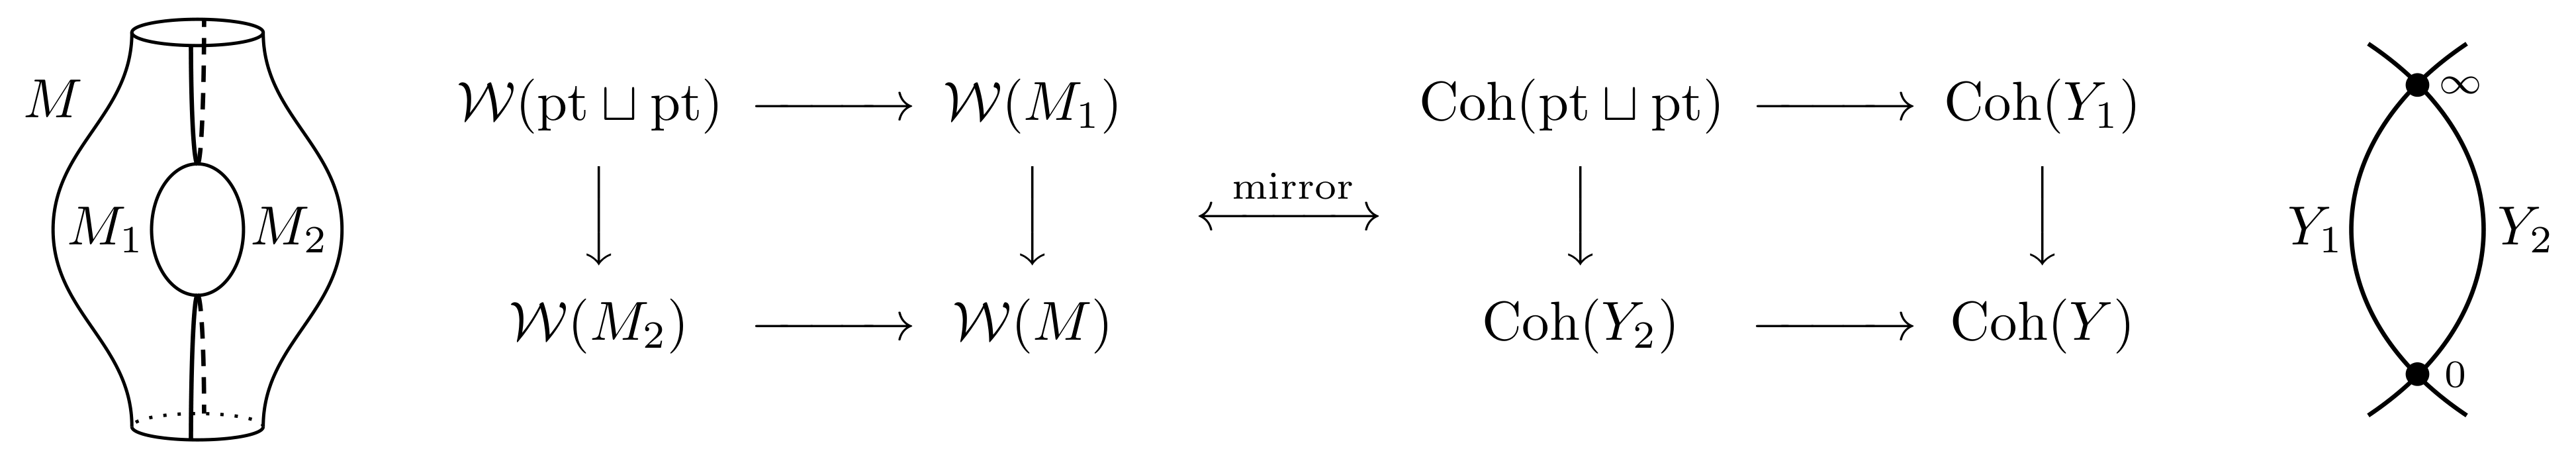
\includegraphics[width=\linewidth]{figures/fig1_twice_punctured_torus_arcs.png}
\caption{例 \ref{ex:3.2} 的扇区分解及其在同调镜像对称下的对应物（原文第 14 页底部；\textbf{原文未编号}，
此处按图 1 编号）。从左至右：带两个 puncture 的环面 $M$ 沿两条弧（虚线）切分为两个刘维尔扇区
$M_1,M_2$；缠绕深谷范畴沿扇区分解的推出图；镜像一侧（$\mathrm{Coh}$ 方向）对应的凝聚层推出图；
以及由 $Y_1,Y_2\simeq\mathbb{P}^{1}$ 在 $\{0,\infty\}$ 处粘合而得的双结点椭圆曲线
$Y=Y_1\cup_{\{0,\infty\}}Y_2$。中间的 $\xrightarrow{\ \text{mirror}\ }$ 标出两侧之间的
同调镜像对称对应关系。}
\label{fig:3.2}
\end{figure}

这一视角对于研究大体积（large volume）极限处的镜像对称特别有用，例如可以用它来理解 Gammage 与 Shende
关于极仿射（very affine）超曲面镜像对称的结果 \cite{r50}。

\paragraph{逆变函子性。}
尽管有上述协变函子性，缠绕深谷范畴关于子区域的包含一般却表现出逆变的行为。
这件事的原型是 Abouzaid 与 Seidel \cite{r12} 所构造的\textbf{限制函子}：从刘维尔流形 $M$ 的
缠绕深谷范畴到刘维尔子区域 $M_-\subset M$（即一个余维 $0$、其凸边界横截于刘维尔向量场的子流形；
$M_-$ 的缠绕深谷范畴定义为它的完备化——刘维尔流形
$\widehat{M}_-=M_-\cup_{\partial M_-}[1,\infty)\times\partial M_-$ ——的缠绕深谷范畴）的
缠绕深谷范畴。这一构造所依赖的几何思想与 Viterbo 早先构造的、从 $M$ 的辛上同调到 $M_-$ 的
辛上同调的限制映射相同 \cite{r103}，即：使用在 $\partial M_-$ 附近增长得非常陡峭的哈密顿函数，
对这样的函数，不存在从 $M\setminus M_-$ 中的生成元到 $M_-$ 中生成元的 Floer 轨道，
于是链层面的限制映射相当于对一个子复形取商（事实上，是对乘积运算而言的一个理想）。

Heather Lee 的学位论文 \cite{r68} 用类似的想法构造了与“把 Riemann 面分解为若干裤子
（在柱面上彼此重叠）”相联系的限制函子，并证明它们给出拉回图。
（虽然 Lee 是在恰当设定下工作的，该结果对闭曲面的深谷范畴也适用 \cite{r25}。）

\begin{thm}[Lee \cite{r68}]\label{thm:3.3}
给定 Riemann 面 $\Sigma$ 沿一条非平凡简单闭曲线（或若干条这样的曲线之并）$\gamma$ 切开所得的
分解 $\Sigma_1\cup_{\gamma}\Sigma_2$，存在从 $\Sigma$ 的缠绕深谷范畴到 $\Sigma_1$、$\Sigma_2$
以及 $\gamma$ 的一个柱状邻域 $C$ 的缠绕深谷范畴的限制函子，它们构成一个拉回图：
\begin{equation}\label{eq:3.3}
\begin{CD}
\WW(\Sigma)  @>>>  \WW(\Sigma_1)\\
@VVV         @VVV\\
\WW(\Sigma_2) @>>> \WW(C)
\end{CD}
\end{equation}
\end{thm}

（一如既往，$\WW(\Sigma_i)$ 与 $\WW(C)$ 指这些子区域之完备化的缠绕深谷范畴。）
Lee 进一步证明：对 $(\C^{*})^{2}$ 中复曲线在热带极限附近的裤子分解，图 \eqref{eq:3.3} 在
镜像对称下对应于镜像的一个自然仿射覆盖所联系的限制函子；也就是说，
通过拉回图计算 $\Sigma$ 中一对拉格朗日子流形的缠绕 Floer 上同调，与通过镜像上的
\v{C}ech 复形计算层上同调是一致的 \cite{r68}。
另见 \cite{r83} 中一个导向非常相似结果的不同视角，它允许进一步的推广以及在更高维的同调镜像
对称中的应用 \cite{r74}。

% [Tutor Note: 含糊点拨。“协变”与“逆变”并存并不矛盾，这一点值得想清楚，因为初读时极易
% 以为作者前后自相矛盾。正确的理解是：
%  · 协变函子性 $i_*: W(M') → W(M)$ 对应“把对象推前”——对开子集的“延拓/诱导表示”，
%    几何上类似层的\textbf{前推} $i_*$（或代数几何中的 pushforward）。
%  · 逆变函子性（限制函子）对应“把对象拉回”——类似层的\textbf{拉回} $i^*$（restriction）。
% 一个层论中本来就同时有 $i_*$ 与 $i^*$，所以深谷范畴同时具有两种函子性并不奇怪；
% 关键在于两者\textbf{不是}互逆的伴随（虽然在好的情形下 $i_*$ 与 $i^*$ 构成伴随对，
% 但这里的方向/存在性依赖于 sector 与 subdomain 的不同几何设定）。
% 换句话说：定理 3.1 的“扇区”与定理 3.3 的“子区域”是两类不同的子对象，
% 前者边界是扇区边界（有 stops 结构），后者边界是凸的（横截于刘维尔场）。
% 把这两个定理当成“矛盾”是本节最常见的误读。]

\begin{exmp}\label{ex:3.4}
如上，考虑一个带两个 puncture 的环面，但这次沿两条简单闭曲线把它分解为两个裤子
$\Sigma_1,\Sigma_2$，二者沿两条柱状颈 $C',C''$ 彼此粘合。裤子镜像于仿射曲线
$\{xy=0\}\subset\mathbb{A}^{2}$（参看例如 \cite[第 3 节]{r23}），而柱面镜像于带 puncture 的
仿射直线 $\mathbb{G}_m=\mathbb{A}^{1}\setminus\{0\}$；缠绕深谷范畴上的限制函子在同调镜像对称下
对应于把 $Y=\mathbb{P}^{1}\cup_{\{0,\infty\}}\mathbb{P}^{1}$ 分解为两张仿射卡 $U_1,U_2$
（分别补掉 $0$ 与补掉 $\infty$）所联系的限制函子，重叠部分为
$U_1\cap U_2\simeq\mathbb{G}_m\sqcup\mathbb{G}_m$。
\end{exmp}

\begin{figure}[htbp]
\centering
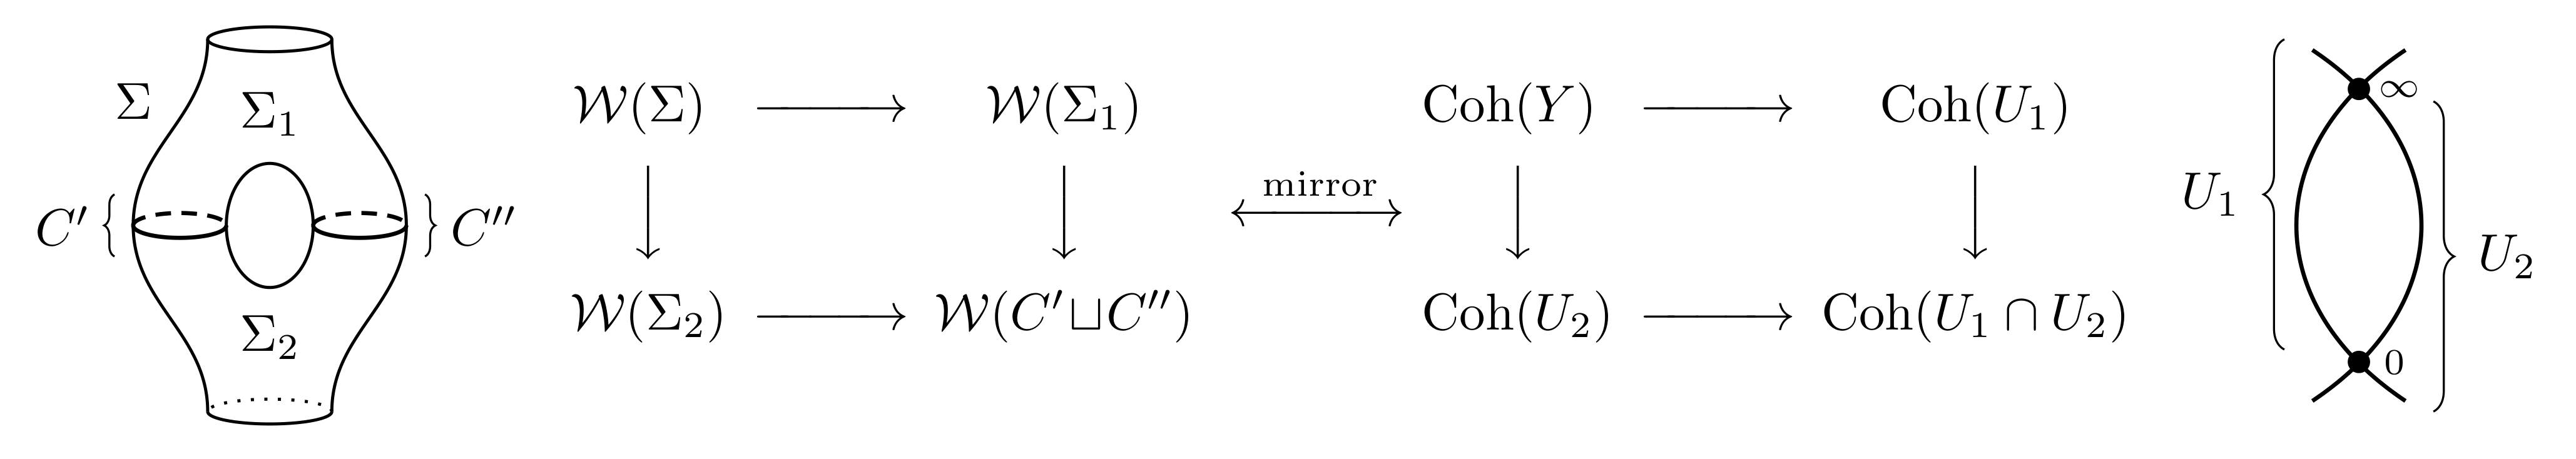
\includegraphics[width=\linewidth]{figures/fig2_twice_punctured_torus_circles.png}
\caption{例 \ref{ex:3.4} 的裤子分解及其镜像对应（原文第 15 页中部；\textbf{原文未编号}，
此处按图 2 编号）。从左至右：带两个 puncture 的环面 $\Sigma$ 沿两条简单闭曲线切分为两个裤子
$\Sigma_1,\Sigma_2$，二者沿两条柱状颈 $C',C''$ 相接；缠绕深谷范畴的拉回图；镜像一侧凝聚层的
拉回图；以及 $Y=\mathbb{P}^{1}\cup_{\{0,\infty\}}\mathbb{P}^{1}$ 由两张仿射卡 $U_1,U_2$
覆盖、重叠为 $\mathbb{G}_m\sqcup\mathbb{G}_m$ 的图示。与图 \ref{fig:3.2} 对照可见：
推出对应粘合、拉回对应覆盖，这是“局部—整体原理”在两套语言中的同一件事。}
\label{fig:3.4}
\end{figure}

% [Tutor Note: 阅读提示。请把图 1 与图 2 并排对照，这是本节最经济的一课：
%  · 图 1（例 3.2，沿弧切）⇒ 中间是\textbf{推出}图，镜像一侧是“粘合”两个 P¹ 得到结点曲线；
%  · 图 2（例 3.4，沿闭曲线切）⇒ 中间是\textbf{拉回}图，镜像一侧是“覆盖”两张仿射卡并作 Čech。
% 同一个几何对象（带两 puncture 的环面）的两种切法，给出两种相反的函子性——因为切法决定了
% 是“沿扇区边界粘合”还是“沿子区域覆盖”。这正是层论中 pushforward / pullback 对偶的几何体现，
% 也解释了为什么“局部—整体原理”不能只有一种形式。]

值得注意的是：当其中一条曲线同伦平凡时（即分解的某一块是圆盘），定理 \ref{thm:3.3} 失效。
的确，此时对足够陡峭的哈密顿函数，Floer 轨道的局部性不再成立：用一个圆盘去封住 $\Sigma_i$
会非平凡地形变其深谷范畴（参看 \S\ref{sec:2.4}），而任何这样的设定下的局部—整体原理都必须
把这个形变纳入其中。

% [Tutor Note: 含糊点拨。这条“失效”的注记是全节最有信息量的一句话，它把 §2.4 与 §3.2 焊在一起：
% 用一个圆盘封住某一块 $\Sigma_i$，相当于对它的深谷范畴作一次形变——这与 §2.4 中的
% （相对 / bulk）形变机制在精神上是同一类操作：封盘引入了新的“包围盘”贡献，从而改变了
% Floer 数据。原文只说 “cf. §2.4”，并未声称这两种形变是同一回事；此处也不宜把补上的圆盘
% 直接等同于某个除子 $D$（圆盘是二维链，而相对深谷范畴的 $D$ 是复余维 1 的对象）。
% 要点在于：“局部—整体原理”的正确形态不是“把局部的范畴粘起来”，而是“把局部的\textbf{形变族}
% 粘起来”——用层论的语言，不是常数层而是带形变参数的层。这一点在 [24] 的“修正族 Floer 复形”
% 与 Groman–Varolgunes 的“相对辛上同调”中被各自形式化，原文在接下来两段正好点出这两个方向。]

在“闭弦”设定下，这一方向上的一个重要概念性步骤是 Groman 与 Varolgunes \cite{r60} 的工作：
他们定义了区域 $V\subset M$ 的\textbf{相对辛上同调} $\SH^{*}_{M}(V)$，它由 $M\setminus V$ 中
连接 $V$ 内生成元的 Floer 解之部分对 $\SH^{*}(V)$ 所作的贡献来形变后者。
（当 $V$ 是 $M$ 中除子 $D$ 的补集时，这相当于把 $M$ 中的 Floer 理论描述为 $M\setminus D$ 中
Floer 理论的一个形变；但这一设定要一般得多，例如允许考虑拉格朗日纤维化 $\pi:M\to B$ 的全空间中
形如 $\pi^{-1}(U)$（$U\subset B$ 适当）的子集。）人们期待，对缠绕深谷范畴也应当存在类似的概念，
并对由子区域覆盖所联系的一族限制函子给出拉回图——即便在局部范畴必须被非局部贡献所形变的
设定下也是如此。

在拉格朗日环面纤维化 $\pi:M\to B$ 的 SYZ 镜像对称设定下，相对辛上同调与相对缠绕深谷范畴
应当关于 $B$ 的适当区域覆盖表现出层的行为。回到 \S\ref{sec:3.1} 末的讨论：
\cite{r24} 中引入的修正族 Floer 复形 $(C,\delta+\{\mu^{0},\cdot\})$ 也应当如此；
事实上，后者应当（在与 $BV$-代数结构相容的意义下）拟同构于相对辛上同调的
\v{C}ech 复形，因为二者都被期待给出修正后镜像上多重向量场或 Hochschild 上链的
\v{C}ech 模型。

% [Tutor Note: 阅读提示（全文收束）。最后这一段其实是在给整篇文章“收口”，把三条线索系在一起：
%   (1) 深谷范畴（开弦，§2）→ 族 Floer / SYZ 镜像（§3.1）→ 修正族 Floer 复形 (C, δ+{μ⁰,·})；
%   (2) 辛上同调（闭弦，§1）→ 相对辛上同调 SH*_M(V)（§3.2）→ 其 Čech 复形；
%   (3) 二者的同调代数对应：多重向量场 / Hochschild 上链。
% “二者都应当给出同一个 Čech 模型”这一句话，是整篇文章的未证猜想中最核心的一条：
% 它断言开弦与闭弦在“Floer 理论的几何”这一层面上是同一种东西。作者写 “should be
% quasi-isomorphic”，语气已尽量克制，但仍属猜测。读到这里应清楚：§3 虽含定理 3.1、3.3 与
% 两个已证的例子，但其\textbf{后半与多处结论}仍是纲领与猜想（尤其是本段这条“同一 Čech 模型”
% 的预期），而非定理——这正是标题 “and back again” 的诚实之处。]

\clearpage
\section*{参考文献}
\addcontentsline{toc}{section}{参考文献}
\begin{thebibliography}{105}
\small
% p04_refs.tex --- reference list of arXiv:2510.22476v1 (105 entries, order as in the original)
\bibitem{r1} M. Abouzaid, \emph{A geometric criterion for generating the Fukaya category}, Publ. Math. IH\'ES, 112 (2010), pp. 191--240.
\bibitem{r2} M. Abouzaid, \emph{A cotangent fibre generates the Fukaya category}, Adv. Math., 228 (2011), pp. 894--939.
\bibitem{r3} M. Abouzaid, \emph{Framed bordism and Lagrangian embeddings of exotic spheres}, Ann. Math., 175 (2012), pp. 71--185.
\bibitem{r4} M. Abouzaid, \emph{Family Floer cohomology and mirror symmetry}, in Vol. II of Proc. International Congress of Mathematicians (Seoul, 2014), 2014, pp. 813--836.
\bibitem{r5} M. Abouzaid, \emph{Homological mirror symmetry without corrections}, J. Amer. Math. Soc., 34 (2021), 1059--1173.
\bibitem{r6} M. Abouzaid and D. Auroux, \emph{Homological mirror symmetry for hypersurfaces in $(\mathbb{C}^*)^n$}, Geom. Topol., 28 (2024), pp. 2825--2914.
\bibitem{r7} M. Abouzaid, D. Auroux, and L. Katzarkov, \emph{Lagrangian fibrations on blowups of toric varieties and mirror symmetry for hypersurfaces}, Publ. Math. IH\'ES, 123 (2016), pp. 199--282.
\bibitem{r8} M. Abouzaid and A. Blumberg, \emph{Arnold conjecture and Morava K-theory}, preprint, 2021, \url{https://arxiv.org/abs/2103.01507}.
\bibitem{r9} M. Abouzaid and N. Bottman, \emph{Functoriality in categorical symplectic geometry}, Bull. Amer. Math. Soc., 61 (2024), pp. 525--608.
\bibitem{r10} M. Abouzaid, Y. Groman, and U. Varolgunes, \emph{Framed $E_2$ structures in Floer theory}, Adv. Math., 450 (2024), 109755.
\bibitem{r11} M. Abouzaid and T. Kragh, \emph{Simple homotopy equivalence of nearby Lagrangians}, Acta Math., 220 (2018), pp. 207--237.
\bibitem{r12} M. Abouzaid and P. Seidel, \emph{An open string analogue of Viterbo functoriality}, Geom. Topol., 14 (2010), pp. 627--718.
\bibitem{r13} M. Abouzaid and I. Smith, \emph{Khovanov homology from Floer cohomology}, J. Amer. Math. Soc., 32 (2019), pp. 1--79.
\bibitem{r14} M. Abouzaid and Z. Sylvan, \emph{Homological mirror symmetry for local SYZ singularities}, preprint, 2021, \url{https://arxiv.org/abs/2107.05068}.
\bibitem{r15} M. Aganagic, \emph{Knot categorification from mirror symmetry, part II: Lagrangians}, Adv. Theor. Math. Phys., 29 (2025), pp. 557--749.
\bibitem{r16} V. Arnol'd, \emph{Sur une propri\'et\'e topologique des applications globalement canoniques de la m\'ecanique classique}, C. R. Acad. Sci. Paris, 261 (1965), pp. 3719--3722.
\bibitem{r17} M. F. Atiyah, \emph{New invariants of 3- and 4-dimensional manifolds}, in The Mathematical Heritage of Hermann Weyl, R. O. Wells, ed., vol. 48 of Proc. Symposia Pure Math., 1988, Amer. Math. Soc., pp. 285--299.
\bibitem{r18} M. Audin and M. Damian, \emph{Th\'eorie de Morse et homologie de Floer}, EDP Sciences, 2010; English transl. \emph{Morse theory and Floer homology}, Universitext, Springer, EDP Sciences, 2014.
\bibitem{r19} D. Auroux, \emph{Mirror symmetry and T-duality in the complement of an anticanonical divisor}, J. G\"okova Geom. Topol., 1 (2007), pp. 51--91.
\bibitem{r20} D. Auroux, \emph{Special Lagrangian fibrations, wall-crossing, and mirror symmetry}, in Vol. 13 of Surveys in Differential Geometry, Intl. Press, 2009, pp. 1--47.
\bibitem{r21} D. Auroux, \emph{Fukaya categories and bordered Heegaard-Floer homology}, in vol. II of Proc. International Congress of Mathematicians (Hyderabad, 2010), Hindustan Book Agency, 2010, pp. 917--941.
\bibitem{r22} D. Auroux, \emph{A beginner's introduction to Fukaya categories}, in Contact and Symplectic Topology, F. Bourgeois et al., eds., vol. 26 of Bolyai Soc. Math. Stud., J\'anos Bolyai Mathematical Society, Budapest, 2014, Springer, Cham, pp. 85--136.
\bibitem{r23} D. Auroux, \emph{Speculations on homological mirror symmetry for hypersurfaces in $(\mathbb{C}^*)^n$}, in Vol. 22 of Surveys in Differential Geometry, Intl. Press, 2018, pp. 1--47.
\bibitem{r24} D. Auroux, \emph{Holomorphic discs of negative Maslov index and extended deformations in mirror symmetry}, preprint, 2023, \url{https://arxiv.org/abs/2309.13010}.
\bibitem{r25} D. Auroux and I. Smith, \emph{Fukaya categories of surfaces, spherical objects, and mapping class groups}, Forum Math. Sigma, 9 (2021), e26, pp. 1--50.
\bibitem{r26} S. Bai and G. Xu, \emph{Arnold conjecture over integers}, preprint, 2022, \url{https://arxiv.org/abs/2209.08599}.
\bibitem{r27} P. Biran and O. Cornea, \emph{A Lagrangian quantum homology}, in New perspectives and challenges in symplectic field theory, vol. 49 of CRM Proc. Lecture Notes, 2009, Amer. Math. Soc., pp. 1--44.
\bibitem{r28} M. S. Borman, M. El Alami, and N. Sheridan, \emph{An $L_\infty$ structure on symplectic cohomology}, preprint, 2024, \url{https://arxiv.org/abs/2408.09163}.
\bibitem{r29} M. S. Borman, M. El Alami, and N. Sheridan, \emph{Maurer-Cartan elements in symplectic cohomology from compactifications}, preprint, 2024, \url{https://arxiv.org/abs/2408.09221}.
\bibitem{r30} A. Cannas da Silva, \emph{Lectures on symplectic geometry}, vol. 1764 of Lecture Notes in Math., Springer, 2001.
\bibitem{r31} B. Chantraine, G. Dimitroglou Rizell, P. Ghiggini, and R. Golovko, \emph{Geometric generation of the wrapped Fukaya category of Weinstein manifolds and sectors}, Ann. Sci. \'Ec. Norm. Sup\'er., 57 (2024), 1--85.
\bibitem{r32} F. Charest and C. T. Woodward, \emph{Floer cohomology and flips}, Mem. Amer. Math. Soc., 279 (2022), no. 1372.
\bibitem{r33} C.-H. Cho, H. Hong, and S.-C. Lau, \emph{Noncommutative homological mirror functor}, Mem. Amer. Math. Soc., 271 (2021), no. 1326.
\bibitem{r34} C.-H. Cho, H. Hong, and S.-C. Lau, \emph{Gluing localizes mirror functors}, J. Differential Geom., 126 (2024), pp. 1001--1095.
\bibitem{r35} C.-H. Cho and Y.-G. Oh, \emph{Floer cohomology and disc instantons of Lagrangian torus fibers in Fano toric manifolds}, Asian J. Math., 10 (2006), pp. 773--814.
\bibitem{r36} A. Daemi, K. Fukaya, and M. Lipyanskiy, \emph{Lagrangians, SO(3) instantons and the Atiyah-Floer conjecture}, preprint, 2021, \url{https://arxiv.org/abs/2109.07032}.
\bibitem{r37} B. Fang, C.-C. M. Liu, D. Treumann, and E. Zaslow, \emph{A categorification of Morelli's theorem}, Invent. Math., 186 (2011), pp. 79--114.
\bibitem{r38} B. Filippenko and K. Wehrheim, \emph{A polyfold proof of the Arnold conjecture}, Selecta Math., 28 (2022), 11.
\bibitem{r39} A. Floer, \emph{Morse theory for Lagrangian intersections}, J. Differential Geom., 28 (1988), pp. 513--547.
\bibitem{r40} A. Floer, \emph{Symplectic fixed points and holomorphic spheres}, Comm. Math. Phys., 120 (1989), pp. 575--611.
\bibitem{r41} K. Fukaya, \emph{Floer homology for families -- a progress report}, in Integrable Systems, Topology, and Physics (Tokyo, 2000), Amer. Math. Soc., Providence, RI, 2002, pp. 33--68.
\bibitem{r42} K. Fukaya, \emph{Cyclic symmetry and adic convergence in Lagrangian Floer theory}, Kyoto J. Math., 50 (2010), pp. 521--590.
\bibitem{r43} K. Fukaya, \emph{Unobstructed immersed Lagrangian correspondence and filtered $A_\infty$ functor}, SIGMA, 21 (2025), paper no. 031.
\bibitem{r44} K. Fukaya, Y.-G. Oh, H. Ohta, and K. Ono, \emph{Lagrangian intersection Floer theory: anomaly and obstruction I and II}, vol. 46 of AMS/IP Studies in Advanced Math., Amer. Math. Soc. and International Press, 2009.
\bibitem{r45} K. Fukaya, Y.-G. Oh, H. Ohta, and K. Ono, \emph{Kuranishi structures and virtual fundamental chains}, Springer Monographs in Mathematics, Springer, 2020.
\bibitem{r46} K. Fukaya and K. Ono, \emph{Arnold conjecture and Gromov-Witten invariants for general symplectic manifolds}, Topology, 38 (1999), pp. 933--1048.
\bibitem{r47} K. Fukaya, P. Seidel, and I. Smith, \emph{The symplectic geometry of cotangent bundles from a categorical viewpoint}, in Homological Mirror Symmetry, vol. 757 of Lect. Notes in Physics, Springer, 2009, pp. 1--26.
\bibitem{r48} B. Gammage, \emph{Local mirror symmetry via SYZ}, Bull. Lond. Math. Soc. 56 (2024), pp. 3181--3195.
\bibitem{r49} B. Gammage and M. Jeffs, \emph{Homological mirror symmetry for functors between Fukaya categories of very affine hypersurfaces}, J. Topol., 18 (2025), paper no. e70012.
\bibitem{r50} B. Gammage and V. Shende, \emph{Mirror symmetry for very affine hypersurfaces}, Acta Math., 229 (2022), pp. 287--346.
\bibitem{r51} B. Gammage and V. Shende, \emph{Homological mirror symmetry at large volume}, Tunis. J. Math., 5 (2023), pp. 31--71.
\bibitem{r52} S. Ganatra, \emph{Symplectic cohomology and duality for the wrapped Fukaya category}, Ph.D. thesis, MIT, 2012, \url{https://arxiv.org/abs/1304.7312}.
\bibitem{r53} S. Ganatra, \emph{Cyclic homology, $S^1$-equivariant Floer cohomology, and Calabi-Yau structures}, Geom. Topol., 27 (2023), pp. 3461--3584.
\bibitem{r54} S. Ganatra, \emph{Structural approaches to Fukaya categories and mirror symmetry}, preprint, to appear in Proc. International Congress of Mathematicians (Philadelphia, 2026).
\bibitem{r55} S. Ganatra, A. Hanlon, J. Hicks, D. Pomerleano, and N. Sheridan, \emph{Homological mirror symmetry for Batyrev mirror pairs}, preprint, 2024, \url{https://arxiv.org/abs/2406.05272}.
\bibitem{r56} S. Ganatra, J. Pardon, and V. Shende, \emph{Covariantly functorial wrapped Floer theory on Liouville sectors}, Publ. Math. IH\'ES, 131 (2020), pp. 73--200.
\bibitem{r57} S. Ganatra, J. Pardon, and V. Shende, \emph{Sectorial descent for wrapped Fukaya categories}, J. Amer. Math. Soc., 37 (2024), pp. 499--635.
\bibitem{r58} S. Ganatra, J. Pardon, and V. Shende, \emph{Microlocal Morse theory of wrapped Fukaya categories}, Ann. Math, 199 (2024), pp. 943--1042.
\bibitem{r59} S. Ganatra, T. Perutz, and N. Sheridan, \emph{Mirror symmetry: from categories to curve counts}, preprint, 2015, \url{https://arxiv.org/abs/1510.03839}.
\bibitem{r60} Y. Groman and U. Varolgunes, \emph{Locality of relative symplectic cohomology for complete embeddings}, Compos. Math., 159 (2023), pp. 2551--2637.
\bibitem{r61} A. Hanlon, \emph{Monodromy of monomially admissible Fukaya-Seidel categories mirror to toric varieties}, Adv. Math., 350 (2019), pp. 662--746.
\bibitem{r62} A. Hanlon and J. Hicks, \emph{Aspects of functoriality in homological mirror symmetry for toric varieties}, Adv. Math., 401 (2022), 108317.
\bibitem{r63} K. Hoek, \emph{A Morse-theoretic approach to family Floer cohomology}, Ph.D. thesis, Harvard University, 2025.
\bibitem{r64} H. Hofer and D. Salamon, \emph{Floer homology and Novikov rings}, in The Floer Memorial Volume, Birkh\"auser, 1995, pp. 483--524.
\bibitem{r65} M. Kontsevich, \emph{Homological algebra of mirror symmetry}, in Proc. International Congress of Mathematicians (Z\"urich, 1994), Birkh\"auser, 1995, pp. 120--139.
\bibitem{r66} M. Kontsevich, \emph{Symplectic geometry of homological algebra}, preprint, 2009, \url{https://www.ihes.fr/~maxim/TEXTS/Symplectic_AT2009.pdf}
\bibitem{r67} T. Large, \emph{Spectral Fukaya categories for Liouville manifolds}, Ph.D. thesis, MIT, 2021.
\bibitem{r68} H. Lee, \emph{Homological mirror symmetry for open Riemann surfaces from pair-of-pants decompositions}, preprint, 2016, \url{https://arxiv.org/abs/1608.04473}.
\bibitem{r69} Y. Lekili and A. Polishchuk, \emph{Homological mirror symmetry for higher-dimensional pairs of pants}, Compositio Math., 156 (2020), pp. 1310--1347.
\bibitem{r70} R. Lipshitz, P. S. Ozsv\'ath, and D. P. Thurston, \emph{Bordered Heegaard Floer homology}, Mem. Amer. Math. Soc., 254 (2018), no. 1216.
\bibitem{r71} G. Liu and G. Tian, \emph{Floer homology and Arnold conjecture}, J. Diff. Geom., 49 (1998), pp. 1--74.
\bibitem{r72} D. McDuff and D. Salamon, \emph{J-holomorphic curves and symplectic topology}, vol. 52 of Amer. Math. Soc. Colloq. Publ., Amer. Math. Soc., 2012.
\bibitem{r73} S. Ma'u, K. Wehrheim, and C. Woodward, \emph{$A_\infty$ functors for Lagrangian correspondences}, Selecta Math., 24 (2018), pp. 1913--2002.
\bibitem{r74} H. Morimura, N. Sibilla, and P. Zhou, \emph{Homological mirror symmetry for complete intersections in algebraic tori}, preprint, 2023, \url{https://arxiv.org/abs/2303.06955}.
\bibitem{r75} D. Nadler, \emph{Microlocal branes are constructible sheaves}, Selecta Math., 15 (2009), pp. 563--619.
\bibitem{r76} D. Nadler, \emph{Wrapped microlocal sheaves on pairs of pants}, preprint, 2016, \url{https://arxiv.org/abs/1604.00114}.
\bibitem{r77} D. Nadler, \emph{Mirror symmetry for the Landau-Ginzburg A-model $M = \mathbb{C}^n$, $W = z_1\cdots z_n$}, Duke Math. J., 168 (2019), pp. 1--84.
\bibitem{r78} D. Nadler and E. Zaslow, \emph{Constructible sheaves and the Fukaya category}, J. Amer. Math. Soc., 22 (2009), pp. 233--286.
\bibitem{r79} Y.-G. Oh, \emph{Floer cohomology of Lagrangian intersections and pseudo-holomorphic disks I and II}, Comm. Pure Appl. Math., 46 (1993), pp. 949--993 and 995--1012.
\bibitem{r80} K. Ono, \emph{On the Arnold conjecture for weakly monotone symplectic manifolds}, Inventiones Math., 119 (1995), pp. 519--537.
\bibitem{r81} P. Ozsv\'ath and Z. Szab\'o, \emph{Holomorphic disks and topological invariants for closed three-manifolds}, Ann. of Math., 159 (2004), pp. 1027--1158.
\bibitem{r82} J. Pardon, \emph{An algebraic approach to virtual fundamental cycles on moduli spaces of pseudo-holomorphic curves}, Geom. Topol., 20 (2016), pp. 779--1034.
\bibitem{r83} J. Pascaleff and N. Sibilla, \emph{Topological Fukaya category and mirror symmetry for punctured surfaces}, Compositio Math., 155 (2019), pp. 599--644.
\bibitem{r84} T. Perutz and N. Sheridan, \emph{Constructing the relative Fukaya category}, J. Symplectic Geom., 21 (2023), pp. 997--1076.
\bibitem{r85} A. Polishchuk and E. Zaslow, \emph{Categorical mirror symmetry: the elliptic curve}, Adv. Theor. Math. Phys., 2 (1998), pp. 443--470.
\bibitem{r86} N. Porcelli and I. Smith, \emph{Bordism of flow modules and exact Lagrangians}, 2024, \url{https://arxiv.org/abs/2401.11766}.
\bibitem{r87} N. Porcelli and I. Smith, \emph{Bordism from quasi-isomorphism}, 2025, \url{https://arxiv.org/abs/2509.21587}.
\bibitem{r88} S. Rezchikov, \emph{Integral Arnol'd conjecture}, preprint, 2022, \url{https://arxiv.org/abs/2209.11165}.
\bibitem{r89} A. F. Ritter and I. Smith, \emph{The monotone wrapped Fukaya category and the open-closed string map}, Selecta Math., 23 (2017), pp. 533--642.
\bibitem{r90} D. A. Salamon and K. Wehrheim, \emph{Instanton Floer homology with Lagrangian boundary conditions}, Geom. Topol., 12 (2008), pp. 747--918.
\bibitem{r91} P. Seidel, \emph{Fukaya categories and deformations}, in Vol. II of Proc. International Congress of Mathematicians (Beijing, 2002), Higher Ed. Press, Beijing, 2002, pp. 351--360.
\bibitem{r92} P. Seidel, \emph{Fukaya categories and Picard-Lefschetz theory}, Zurich Lect. in Adv. Math., European Math. Soc., Z\"urich, 2008.
\bibitem{r93} P. Seidel, \emph{Fukaya $A_\infty$-structures associated to Lefschetz fibrations I}, J. Symplectic Geom., 10 (2012), pp. 325--388.
\bibitem{r94} P. Seidel, \emph{Homological mirror symmetry for the genus two curve}, J. Algebraic Geom., 20 (2011), 727--769.
\bibitem{r95} N. Sheridan, \emph{Homological mirror symmetry for Calabi-Yau hypersurfaces in projective space}, Inventiones Math., 199 (2015), pp. 1--186.
\bibitem{r96} J. P. Solomon and S. B. Tukachinsky, \emph{Differential forms, Fukaya $A_\infty$ algebras, and Gromov-Witten axioms}, J. Symplectic Geom., 20 (2022), pp. 927--994.
\bibitem{r97} A. Strominger, S.-T. Yau, and E. Zaslow, \emph{Mirror symmetry is T-duality}, Nucl. Phys. B, 479 (1996), pp. 243--259.
\bibitem{r98} Z. Sylvan, \emph{On partially wrapped Fukaya categories}, J. Topol., 12 (2019), pp. 372--441.
\bibitem{r99} Z. Sylvan, \emph{Orlov and Viterbo functors in partially wrapped Fukaya categories}, 2019, \url{https://arxiv.org/abs/1908.02317}.
\bibitem{r100} J. Tu, \emph{On the reconstruction problem in mirror symmetry}, Adv. Math., 256 (2014), pp. 449--478.
\bibitem{r101} K. Ueda, \emph{On the Fukaya categories of projective hypersurfaces of general type}, preprint, 2025, \url{https://arxiv.org/abs/2505.00910}.
\bibitem{r102} R. Vianna, \emph{Infinitely many exotic monotone Lagrangian tori in $\mathbb{C}P^2$}, J. Topol., 9 (2016), pp. 535--551.
\bibitem{r103} C. Viterbo, \emph{Functors and computations in Floer cohomology with applications, Part I}, Geom. Funct. Anal., 9 (1999), pp. 985--1033.
\bibitem{r104} J. Weber, \emph{Three approaches towards Floer homology of cotangent bundles}, J. Symplectic Geom., 3 (2005), pp. 671--701.
\bibitem{r105} H. Yuan, \emph{Family Floer program and non-archimedean SYZ mirror construction}, preprint, 2020, \url{https://arxiv.org/abs/2003.06106}.
\end{thebibliography}

\end{document}
